
\documentclass{article} % For LaTeX2e
\usepackage{iclr2024_conference,times}

% Optional math commands from https://github.com/goodfeli/dlbook_notation.
%%%%% NEW MATH DEFINITIONS %%%%%

\usepackage{amsmath,amsfonts,bm}

% Mark sections of captions for referring to divisions of figures
\newcommand{\figleft}{{\em (Left)}}
\newcommand{\figcenter}{{\em (Center)}}
\newcommand{\figright}{{\em (Right)}}
\newcommand{\figtop}{{\em (Top)}}
\newcommand{\figbottom}{{\em (Bottom)}}
\newcommand{\captiona}{{\em (a)}}
\newcommand{\captionb}{{\em (b)}}
\newcommand{\captionc}{{\em (c)}}
\newcommand{\captiond}{{\em (d)}}

% Highlight a newly defined term
\newcommand{\newterm}[1]{{\bf #1}}


% Figure reference, lower-case.
\def\figref#1{figure~\ref{#1}}
% Figure reference, capital. For start of sentence
\def\Figref#1{Figure~\ref{#1}}
\def\twofigref#1#2{figures \ref{#1} and \ref{#2}}
\def\quadfigref#1#2#3#4{figures \ref{#1}, \ref{#2}, \ref{#3} and \ref{#4}}
% Section reference, lower-case.
\def\secref#1{section~\ref{#1}}
% Section reference, capital.
\def\Secref#1{Section~\ref{#1}}
% Reference to two sections.
\def\twosecrefs#1#2{sections \ref{#1} and \ref{#2}}
% Reference to three sections.
\def\secrefs#1#2#3{sections \ref{#1}, \ref{#2} and \ref{#3}}
% Reference to an equation, lower-case.
\def\eqref#1{equation~\ref{#1}}
% Reference to an equation, upper case
\def\Eqref#1{Equation~\ref{#1}}
% A raw reference to an equation---avoid using if possible
\def\plaineqref#1{\ref{#1}}
% Reference to a chapter, lower-case.
\def\chapref#1{chapter~\ref{#1}}
% Reference to an equation, upper case.
\def\Chapref#1{Chapter~\ref{#1}}
% Reference to a range of chapters
\def\rangechapref#1#2{chapters\ref{#1}--\ref{#2}}
% Reference to an algorithm, lower-case.
\def\algref#1{algorithm~\ref{#1}}
% Reference to an algorithm, upper case.
\def\Algref#1{Algorithm~\ref{#1}}
\def\twoalgref#1#2{algorithms \ref{#1} and \ref{#2}}
\def\Twoalgref#1#2{Algorithms \ref{#1} and \ref{#2}}
% Reference to a part, lower case
\def\partref#1{part~\ref{#1}}
% Reference to a part, upper case
\def\Partref#1{Part~\ref{#1}}
\def\twopartref#1#2{parts \ref{#1} and \ref{#2}}

\def\ceil#1{\lceil #1 \rceil}
\def\floor#1{\lfloor #1 \rfloor}
\def\1{\bm{1}}
\newcommand{\train}{\mathcal{D}}
\newcommand{\valid}{\mathcal{D_{\mathrm{valid}}}}
\newcommand{\test}{\mathcal{D_{\mathrm{test}}}}

\def\eps{{\epsilon}}


% Random variables
\def\reta{{\textnormal{$\eta$}}}
\def\ra{{\textnormal{a}}}
\def\rb{{\textnormal{b}}}
\def\rc{{\textnormal{c}}}
\def\rd{{\textnormal{d}}}
\def\re{{\textnormal{e}}}
\def\rf{{\textnormal{f}}}
\def\rg{{\textnormal{g}}}
\def\rh{{\textnormal{h}}}
\def\ri{{\textnormal{i}}}
\def\rj{{\textnormal{j}}}
\def\rk{{\textnormal{k}}}
\def\rl{{\textnormal{l}}}
% rm is already a command, just don't name any random variables m
\def\rn{{\textnormal{n}}}
\def\ro{{\textnormal{o}}}
\def\rp{{\textnormal{p}}}
\def\rq{{\textnormal{q}}}
\def\rr{{\textnormal{r}}}
\def\rs{{\textnormal{s}}}
\def\rt{{\textnormal{t}}}
\def\ru{{\textnormal{u}}}
\def\rv{{\textnormal{v}}}
\def\rw{{\textnormal{w}}}
\def\rx{{\textnormal{x}}}
\def\ry{{\textnormal{y}}}
\def\rz{{\textnormal{z}}}

% Random vectors
\def\rvepsilon{{\mathbf{\epsilon}}}
\def\rvtheta{{\mathbf{\theta}}}
\def\rva{{\mathbf{a}}}
\def\rvb{{\mathbf{b}}}
\def\rvc{{\mathbf{c}}}
\def\rvd{{\mathbf{d}}}
\def\rve{{\mathbf{e}}}
\def\rvf{{\mathbf{f}}}
\def\rvg{{\mathbf{g}}}
\def\rvh{{\mathbf{h}}}
\def\rvu{{\mathbf{i}}}
\def\rvj{{\mathbf{j}}}
\def\rvk{{\mathbf{k}}}
\def\rvl{{\mathbf{l}}}
\def\rvm{{\mathbf{m}}}
\def\rvn{{\mathbf{n}}}
\def\rvo{{\mathbf{o}}}
\def\rvp{{\mathbf{p}}}
\def\rvq{{\mathbf{q}}}
\def\rvr{{\mathbf{r}}}
\def\rvs{{\mathbf{s}}}
\def\rvt{{\mathbf{t}}}
\def\rvu{{\mathbf{u}}}
\def\rvv{{\mathbf{v}}}
\def\rvw{{\mathbf{w}}}
\def\rvx{{\mathbf{x}}}
\def\rvy{{\mathbf{y}}}
\def\rvz{{\mathbf{z}}}

% Elements of random vectors
\def\erva{{\textnormal{a}}}
\def\ervb{{\textnormal{b}}}
\def\ervc{{\textnormal{c}}}
\def\ervd{{\textnormal{d}}}
\def\erve{{\textnormal{e}}}
\def\ervf{{\textnormal{f}}}
\def\ervg{{\textnormal{g}}}
\def\ervh{{\textnormal{h}}}
\def\ervi{{\textnormal{i}}}
\def\ervj{{\textnormal{j}}}
\def\ervk{{\textnormal{k}}}
\def\ervl{{\textnormal{l}}}
\def\ervm{{\textnormal{m}}}
\def\ervn{{\textnormal{n}}}
\def\ervo{{\textnormal{o}}}
\def\ervp{{\textnormal{p}}}
\def\ervq{{\textnormal{q}}}
\def\ervr{{\textnormal{r}}}
\def\ervs{{\textnormal{s}}}
\def\ervt{{\textnormal{t}}}
\def\ervu{{\textnormal{u}}}
\def\ervv{{\textnormal{v}}}
\def\ervw{{\textnormal{w}}}
\def\ervx{{\textnormal{x}}}
\def\ervy{{\textnormal{y}}}
\def\ervz{{\textnormal{z}}}

% Random matrices
\def\rmA{{\mathbf{A}}}
\def\rmB{{\mathbf{B}}}
\def\rmC{{\mathbf{C}}}
\def\rmD{{\mathbf{D}}}
\def\rmE{{\mathbf{E}}}
\def\rmF{{\mathbf{F}}}
\def\rmG{{\mathbf{G}}}
\def\rmH{{\mathbf{H}}}
\def\rmI{{\mathbf{I}}}
\def\rmJ{{\mathbf{J}}}
\def\rmK{{\mathbf{K}}}
\def\rmL{{\mathbf{L}}}
\def\rmM{{\mathbf{M}}}
\def\rmN{{\mathbf{N}}}
\def\rmO{{\mathbf{O}}}
\def\rmP{{\mathbf{P}}}
\def\rmQ{{\mathbf{Q}}}
\def\rmR{{\mathbf{R}}}
\def\rmS{{\mathbf{S}}}
\def\rmT{{\mathbf{T}}}
\def\rmU{{\mathbf{U}}}
\def\rmV{{\mathbf{V}}}
\def\rmW{{\mathbf{W}}}
\def\rmX{{\mathbf{X}}}
\def\rmY{{\mathbf{Y}}}
\def\rmZ{{\mathbf{Z}}}

% Elements of random matrices
\def\ermA{{\textnormal{A}}}
\def\ermB{{\textnormal{B}}}
\def\ermC{{\textnormal{C}}}
\def\ermD{{\textnormal{D}}}
\def\ermE{{\textnormal{E}}}
\def\ermF{{\textnormal{F}}}
\def\ermG{{\textnormal{G}}}
\def\ermH{{\textnormal{H}}}
\def\ermI{{\textnormal{I}}}
\def\ermJ{{\textnormal{J}}}
\def\ermK{{\textnormal{K}}}
\def\ermL{{\textnormal{L}}}
\def\ermM{{\textnormal{M}}}
\def\ermN{{\textnormal{N}}}
\def\ermO{{\textnormal{O}}}
\def\ermP{{\textnormal{P}}}
\def\ermQ{{\textnormal{Q}}}
\def\ermR{{\textnormal{R}}}
\def\ermS{{\textnormal{S}}}
\def\ermT{{\textnormal{T}}}
\def\ermU{{\textnormal{U}}}
\def\ermV{{\textnormal{V}}}
\def\ermW{{\textnormal{W}}}
\def\ermX{{\textnormal{X}}}
\def\ermY{{\textnormal{Y}}}
\def\ermZ{{\textnormal{Z}}}

% Vectors
\def\vzero{{\bm{0}}}
\def\vone{{\bm{1}}}
\def\vmu{{\bm{\mu}}}
\def\vtheta{{\bm{\theta}}}
\def\va{{\bm{a}}}
\def\vb{{\bm{b}}}
\def\vc{{\bm{c}}}
\def\vd{{\bm{d}}}
\def\ve{{\bm{e}}}
\def\vf{{\bm{f}}}
\def\vg{{\bm{g}}}
\def\vh{{\bm{h}}}
\def\vi{{\bm{i}}}
\def\vj{{\bm{j}}}
\def\vk{{\bm{k}}}
\def\vl{{\bm{l}}}
\def\vm{{\bm{m}}}
\def\vn{{\bm{n}}}
\def\vo{{\bm{o}}}
\def\vp{{\bm{p}}}
\def\vq{{\bm{q}}}
\def\vr{{\bm{r}}}
\def\vs{{\bm{s}}}
\def\vt{{\bm{t}}}
\def\vu{{\bm{u}}}
\def\vv{{\bm{v}}}
\def\vw{{\bm{w}}}
\def\vx{{\bm{x}}}
\def\vy{{\bm{y}}}
\def\vz{{\bm{z}}}

% Elements of vectors
\def\evalpha{{\alpha}}
\def\evbeta{{\beta}}
\def\evepsilon{{\epsilon}}
\def\evlambda{{\lambda}}
\def\evomega{{\omega}}
\def\evmu{{\mu}}
\def\evpsi{{\psi}}
\def\evsigma{{\sigma}}
\def\evtheta{{\theta}}
\def\eva{{a}}
\def\evb{{b}}
\def\evc{{c}}
\def\evd{{d}}
\def\eve{{e}}
\def\evf{{f}}
\def\evg{{g}}
\def\evh{{h}}
\def\evi{{i}}
\def\evj{{j}}
\def\evk{{k}}
\def\evl{{l}}
\def\evm{{m}}
\def\evn{{n}}
\def\evo{{o}}
\def\evp{{p}}
\def\evq{{q}}
\def\evr{{r}}
\def\evs{{s}}
\def\evt{{t}}
\def\evu{{u}}
\def\evv{{v}}
\def\evw{{w}}
\def\evx{{x}}
\def\evy{{y}}
\def\evz{{z}}

% Matrix
\def\mA{{\bm{A}}}
\def\mB{{\bm{B}}}
\def\mC{{\bm{C}}}
\def\mD{{\bm{D}}}
\def\mE{{\bm{E}}}
\def\mF{{\bm{F}}}
\def\mG{{\bm{G}}}
\def\mH{{\bm{H}}}
\def\mI{{\bm{I}}}
\def\mJ{{\bm{J}}}
\def\mK{{\bm{K}}}
\def\mL{{\bm{L}}}
\def\mM{{\bm{M}}}
\def\mN{{\bm{N}}}
\def\mO{{\bm{O}}}
\def\mP{{\bm{P}}}
\def\mQ{{\bm{Q}}}
\def\mR{{\bm{R}}}
\def\mS{{\bm{S}}}
\def\mT{{\bm{T}}}
\def\mU{{\bm{U}}}
\def\mV{{\bm{V}}}
\def\mW{{\bm{W}}}
\def\mX{{\bm{X}}}
\def\mY{{\bm{Y}}}
\def\mZ{{\bm{Z}}}
\def\mBeta{{\bm{\beta}}}
\def\mPhi{{\bm{\Phi}}}
\def\mLambda{{\bm{\Lambda}}}
\def\mSigma{{\bm{\Sigma}}}

% Tensor
\DeclareMathAlphabet{\mathsfit}{\encodingdefault}{\sfdefault}{m}{sl}
\SetMathAlphabet{\mathsfit}{bold}{\encodingdefault}{\sfdefault}{bx}{n}
\newcommand{\tens}[1]{\bm{\mathsfit{#1}}}
\def\tA{{\tens{A}}}
\def\tB{{\tens{B}}}
\def\tC{{\tens{C}}}
\def\tD{{\tens{D}}}
\def\tE{{\tens{E}}}
\def\tF{{\tens{F}}}
\def\tG{{\tens{G}}}
\def\tH{{\tens{H}}}
\def\tI{{\tens{I}}}
\def\tJ{{\tens{J}}}
\def\tK{{\tens{K}}}
\def\tL{{\tens{L}}}
\def\tM{{\tens{M}}}
\def\tN{{\tens{N}}}
\def\tO{{\tens{O}}}
\def\tP{{\tens{P}}}
\def\tQ{{\tens{Q}}}
\def\tR{{\tens{R}}}
\def\tS{{\tens{S}}}
\def\tT{{\tens{T}}}
\def\tU{{\tens{U}}}
\def\tV{{\tens{V}}}
\def\tW{{\tens{W}}}
\def\tX{{\tens{X}}}
\def\tY{{\tens{Y}}}
\def\tZ{{\tens{Z}}}


% Graph
\def\gA{{\mathcal{A}}}
\def\gB{{\mathcal{B}}}
\def\gC{{\mathcal{C}}}
\def\gD{{\mathcal{D}}}
\def\gE{{\mathcal{E}}}
\def\gF{{\mathcal{F}}}
\def\gG{{\mathcal{G}}}
\def\gH{{\mathcal{H}}}
\def\gI{{\mathcal{I}}}
\def\gJ{{\mathcal{J}}}
\def\gK{{\mathcal{K}}}
\def\gL{{\mathcal{L}}}
\def\gM{{\mathcal{M}}}
\def\gN{{\mathcal{N}}}
\def\gO{{\mathcal{O}}}
\def\gP{{\mathcal{P}}}
\def\gQ{{\mathcal{Q}}}
\def\gR{{\mathcal{R}}}
\def\gS{{\mathcal{S}}}
\def\gT{{\mathcal{T}}}
\def\gU{{\mathcal{U}}}
\def\gV{{\mathcal{V}}}
\def\gW{{\mathcal{W}}}
\def\gX{{\mathcal{X}}}
\def\gY{{\mathcal{Y}}}
\def\gZ{{\mathcal{Z}}}

% Sets
\def\sA{{\mathbb{A}}}
\def\sB{{\mathbb{B}}}
\def\sC{{\mathbb{C}}}
\def\sD{{\mathbb{D}}}
% Don't use a set called E, because this would be the same as our symbol
% for expectation.
\def\sF{{\mathbb{F}}}
\def\sG{{\mathbb{G}}}
\def\sH{{\mathbb{H}}}
\def\sI{{\mathbb{I}}}
\def\sJ{{\mathbb{J}}}
\def\sK{{\mathbb{K}}}
\def\sL{{\mathbb{L}}}
\def\sM{{\mathbb{M}}}
\def\sN{{\mathbb{N}}}
\def\sO{{\mathbb{O}}}
\def\sP{{\mathbb{P}}}
\def\sQ{{\mathbb{Q}}}
\def\sR{{\mathbb{R}}}
\def\sS{{\mathbb{S}}}
\def\sT{{\mathbb{T}}}
\def\sU{{\mathbb{U}}}
\def\sV{{\mathbb{V}}}
\def\sW{{\mathbb{W}}}
\def\sX{{\mathbb{X}}}
\def\sY{{\mathbb{Y}}}
\def\sZ{{\mathbb{Z}}}

% Entries of a matrix
\def\emLambda{{\Lambda}}
\def\emA{{A}}
\def\emB{{B}}
\def\emC{{C}}
\def\emD{{D}}
\def\emE{{E}}
\def\emF{{F}}
\def\emG{{G}}
\def\emH{{H}}
\def\emI{{I}}
\def\emJ{{J}}
\def\emK{{K}}
\def\emL{{L}}
\def\emM{{M}}
\def\emN{{N}}
\def\emO{{O}}
\def\emP{{P}}
\def\emQ{{Q}}
\def\emR{{R}}
\def\emS{{S}}
\def\emT{{T}}
\def\emU{{U}}
\def\emV{{V}}
\def\emW{{W}}
\def\emX{{X}}
\def\emY{{Y}}
\def\emZ{{Z}}
\def\emSigma{{\Sigma}}

% entries of a tensor
% Same font as tensor, without \bm wrapper
\newcommand{\etens}[1]{\mathsfit{#1}}
\def\etLambda{{\etens{\Lambda}}}
\def\etA{{\etens{A}}}
\def\etB{{\etens{B}}}
\def\etC{{\etens{C}}}
\def\etD{{\etens{D}}}
\def\etE{{\etens{E}}}
\def\etF{{\etens{F}}}
\def\etG{{\etens{G}}}
\def\etH{{\etens{H}}}
\def\etI{{\etens{I}}}
\def\etJ{{\etens{J}}}
\def\etK{{\etens{K}}}
\def\etL{{\etens{L}}}
\def\etM{{\etens{M}}}
\def\etN{{\etens{N}}}
\def\etO{{\etens{O}}}
\def\etP{{\etens{P}}}
\def\etQ{{\etens{Q}}}
\def\etR{{\etens{R}}}
\def\etS{{\etens{S}}}
\def\etT{{\etens{T}}}
\def\etU{{\etens{U}}}
\def\etV{{\etens{V}}}
\def\etW{{\etens{W}}}
\def\etX{{\etens{X}}}
\def\etY{{\etens{Y}}}
\def\etZ{{\etens{Z}}}

% The true underlying data generating distribution
\newcommand{\pdata}{p_{\rm{data}}}
% The empirical distribution defined by the training set
\newcommand{\ptrain}{\hat{p}_{\rm{data}}}
\newcommand{\Ptrain}{\hat{P}_{\rm{data}}}
% The model distribution
\newcommand{\pmodel}{p_{\rm{model}}}
\newcommand{\Pmodel}{P_{\rm{model}}}
\newcommand{\ptildemodel}{\tilde{p}_{\rm{model}}}
% Stochastic autoencoder distributions
\newcommand{\pencode}{p_{\rm{encoder}}}
\newcommand{\pdecode}{p_{\rm{decoder}}}
\newcommand{\precons}{p_{\rm{reconstruct}}}

\newcommand{\laplace}{\mathrm{Laplace}} % Laplace distribution

\newcommand{\E}{\mathbb{E}}
\newcommand{\Ls}{\mathcal{L}}
\newcommand{\R}{\mathbb{R}}
\newcommand{\emp}{\tilde{p}}
\newcommand{\lr}{\alpha}
\newcommand{\reg}{\lambda}
\newcommand{\rect}{\mathrm{rectifier}}
\newcommand{\softmax}{\mathrm{softmax}}
\newcommand{\sigmoid}{\sigma}
\newcommand{\softplus}{\zeta}
\newcommand{\KL}{D_{\mathrm{KL}}}
\newcommand{\Var}{\mathrm{Var}}
\newcommand{\standarderror}{\mathrm{SE}}
\newcommand{\Cov}{\mathrm{Cov}}
% Wolfram Mathworld says $L^2$ is for function spaces and $\ell^2$ is for vectors
% But then they seem to use $L^2$ for vectors throughout the site, and so does
% wikipedia.
\newcommand{\normlzero}{L^0}
\newcommand{\normlone}{L^1}
\newcommand{\normltwo}{L^2}
\newcommand{\normlp}{L^p}
\newcommand{\normmax}{L^\infty}

\newcommand{\parents}{Pa} % See usage in notation.tex. Chosen to match Daphne's book.

\DeclareMathOperator*{\argmax}{arg\,max}
\DeclareMathOperator*{\argmin}{arg\,min}

\DeclareMathOperator{\sign}{sign}
\DeclareMathOperator{\Tr}{Tr}
\let\ab\allowbreak


\usepackage{hyperref}
\usepackage{url}
\usepackage{amsmath, amssymb, amsthm}
\usepackage{algorithm}
\usepackage{algpseudocode}
\usepackage{graphicx}
\usepackage{booktabs}
\usepackage{tabularx}
\usepackage{subfigure}


\newtheorem{definition}{Definition} 
\newtheorem{theorem}{Theorem}

\newcommand*{\horzbar}{\rule[.5ex]{2.5ex}{0.5pt}}

% \title{What's the Magic Word? Prompt-Based Controllability of LLMs}
% \title{Magic Words: Toward a Control Theory of LLM Prompting}
\title{\textit{What's the Magic Word?} A Control Theory of LLM Prompting}

% Authors must not appear in the submitted version. They should be hidden
% as long as the \iclrfinalcopy macro remains commented out below.
% Non-anonymous submissions will be rejected without review.

\author{Aman Bhargava$^1$, Cameron Witkowski$^2$, Manav Shah$^2$, Matt Thomson$^1$ 
\thanks{Code will be made available at \texttt{\href{https://github.com/amanb2000/Magic_Words}{https://github.com/amanb2000/Magic\_Words}}.} 
\\
$^1$California Institute of Technology, $^2$University of Toronto \\
\texttt{\{abhargav,mthomson\}@caltech.edu} \\
\texttt{\{cameron.witkowski,manav.shah\}@mail.utoronto.ca} \\ 
}

% The \author macro works with any number of authors. There are two commands
% used to separate the names and addresses of multiple authors: \And and \AND.
%
% Using \And between authors leaves it to \LaTeX{} to determine where to break
% the lines. Using \AND forces a linebreak at that point. So, if \LaTeX{}
% puts 3 of 4 authors names on the first line, and the last on the second
% line, try using \AND instead of \And before the third author name.

\newcommand{\fix}{\marginpar{FIX}}
\newcommand{\new}{\marginpar{NEW}}

\iclrfinalcopy % Uncomment for camera-ready version, but NOT for submission.
\begin{document}


\maketitle

\begin{abstract}
Prompt engineering is crucial for deploying LLMs but is poorly understood mathematically. We formalize LLM systems as a class of discrete stochastic dynamical systems to explore prompt engineering through the lens of control theory. We investigate the reachable set of output token sequences $\mathcal R_y(\mathbf x_0)$ for which there exists a control input sequence $\mathbf u$ for each $\mathbf y \in \mathcal R_y(\mathbf x_0)$ that steers the LLM to output $\mathbf y$ from initial state sequence $\mathbf x_0$.
We offer analytic analysis on the limitations on the controllability of self-attention in terms of reachable set, where we prove an upper bound on the reachable set of outputs $\mathcal R_y(\mathbf x_0)$ as a function of the singular values of the parameter matrices.
We present complementary empirical analysis on the controllability of a panel of LLMs, including Falcon-7b, Llama-7b, and Falcon-40b. 
Our results demonstrate a lower bound on the reachable set of outputs $\mathcal R_y(\mathbf x_0)$ w.r.t. initial state sequences $\mathbf x_0$ sampled from the Wikitext dataset.
We find that the correct next Wikitext token following sequence $\mathbf x_0$ is reachable over 97\% of the time with prompts of $k\leq 10$ tokens. 
We also establish that the top 75 most likely next tokens, as estimated by the LLM itself, are reachable at least 85\% of the time with prompts of $k\leq 10$ tokens. 
Intriguingly, short prompt sequences can dramatically alter the likelihood of specific outputs, even making the least likely tokens become the most likely ones. 
This control-centric analysis of LLMs demonstrates the significant and poorly understood role of input sequences in steering output probabilities, offering a foundational perspective for enhancing language model system capabilities.
\end{abstract}





\section{Introduction}
% LLMs are awesome. Zero-shot deserves to be better understood. 
LLMs pre-trained on unsupervised next token prediction objectives exhibit unprecedented dynamic reprogrammability achieved through ``prompting'', often referred to as zero-shot learning \citep{gpt3, wei2022emergent, hagendorff2023machine, noever2023numeracy, openai2023gpt4, GPT3_5_blog}. 
These capabilities appear to emerge as the model's size, training data, and training time are scaled.
The dynamic reprogrammability of LLMs is akin to the adaptable computational capacities observed in biological systems. 
This feature finds applications across domains such as machine translation \citep{wang2023document}, code generation \citep{code_llama}, and chatbots \cite{rlhf_chatbot}. 
A rigorous understanding of the prompt's influence over LLM generation would be of great utility for understanding LLMs and building more robust and capable systems leveraging LLMs. 


Strategies for controlling pre-trained LLM generation today fall into three broad categories \citep{survey_controllable_text_gen}: 
\begin{enumerate}
    \item \textbf{Input Optimization (Prompting): } Adjusting the input tokens (e.g., rewording the prompt) to improve subsequent text generation. 
    \item \textbf{Model Optimization: } Adjusting the weights of the network (e.g., fine-tuning, RLHF) to improve model behavior during inference. 
    \item \textbf{Post-processing: } Adjusting or re-ranking generated text (e.g., surrogate ranking algorithm). 
\end{enumerate}

Of all these approaches, input optimization (i.e., prompting) is the least invasive and lowest-cost method -- and the least understood.
Prompt optimization is also deeply connected to the zero-shot capabilities of LLMs -- the mysterious emergent capabilities of LLMs such as problem-solving, knowledge retrieval, reasoning, and apparent general intelligence \citep{bubeck2023sparks}. With such a view, we seek to characterize the controllability of LLMs via prompting. 


%Reviewers: Why? Whats the fundamental and applied question? Whats the critical insight that enabled the advance? By framing prompting as a control problem, we define a concept e-k-control and also formulate a mathematical problem that can be analyzed analytically for a single-attention head. 
\subsection{Contribution}

We formalize LLM systems in the mathematical framework of control theory in Section~\ref{sec:ctrl_theory_llms}.
% , exploring notions of reachability and controllability. 
Our analysis focuses on the reachable set of outputs $\mathcal R_y (\mathbf x_0)$ for an LLM system.
% (cf. Definitions~\ref{def:system},~\ref{def:llm-system},~\ref{def:reachable-output-set},~\ref{def:llm-reachable-output-set}). % TODO: Make sure that the second definition reference works. 
The reachable set is a fundamental concept in control theory that underlies notions of controllability, stability, and observability (cf. Appendix~\ref{sec:definitions_ctrl}). 
The reachable output set $R_y(\mathbf x_0)$ is the set of output sequences $\mathbf y$ for which there exists a control input sequence $\mathbf u^*$ that steers the LLM from initial state $\mathbf x_0$ to output $\mathbf y$ (cf. Definitions~\ref{def:llm-reachable-output-set},~\ref{def:reachable-output-set}). 
% We analyze the reachable output set in two ways: 
% (1) we analytically establish necessary conditions for reachability of the self-attention head in Section~\ref{sec:single_head}, and 
% (2) we empirically establish sufficient conditions for reachability on a dataset of initial state sequences $x_0$ sampled from the Wikitext dataset in Section~\ref{sec:results}.

Our analytic results in Section~\ref{sec:single_head} prove an upper bound on the contents of the reachable output set for a self-attention head as a function of the singular values of its parameter matrices. 
Since self-attention is the only component in a transformer block where significant information is exchanged between token representations, this bound provides a foothold for analysis of LLM controllability from the perspective of mechanistic interpretability (e.g., \cite{bricken2023monosemanticity, chefer2021transformer, conmy2023automated}). Moreover, this bound represents a necessary condition for an output to be in the reachable set.

Our empirical results apply state-of-the-art prompt optimization techniques (Section~\ref{sec:methods}) to demonstrate a lower bound on the contents of the reachable output set for a panel of LLMs, including Llama-7b \citep{llama_1}, Falcon-7b, and Falcon-40b \citep{falcon40b}.
Specifically, we sample initial states $\mathbf x_0$ from the Wikitext dataset \citep{wikitext} and probe the reachable output tokens $y$ under length-constrained control input sequences $\mathbf u: |\mathbf u| \leq k$. 
The length constraint $k$ is highly relevant for \textit{optimal control} of LLMs, as prompts with fewer tokens require fewer computation and memory resources. 
We find that the reachable output set contains the ``correct'' next Wikitext token following $\mathbf x_0$ over 97\% of the time with prompts of $k\leq 10$ tokens. We expand our analysis of the contents of $R_y(\mathbf x_0)$ by sampling target output tokens $y$ based on the LLMs initial estimate of output likelihood $P_{LM}(y | \mathbf x_0)$. 
We find that the top 75 most likely output tokens $y$ are reachable at least 85\% of the time with prompts of $k\leq 10$ tokens. 
Intriguingly, some tokens drawn from the set of \textit{least} likely outputs are controllable to the most likely output with $k\leq 4$ control input tokens. 
Our results suggest that prior likelihood-based metrics, such as cross-entropy loss, cannot guarantee exclusion from the reachable set, emphasizing the gap in our current understanding of LLM systems and control. Implications of our results and open questions in LLM control theory are further discussed in Section~\ref{sec:discussion}.

\section{Related Work}
%Fundamental question about whether 'optimal prompts exist' for all inputs and all models. How controllability varies between architectures? Is LLAMA easier or more difficult to prompt than Falcon? what fraction instances  can be 'solved' with prompts ? How does vary? 

%Classes of related work (1) Algorithims for discovering/computing optimal prompts for specific inputs. Gradient, whatever whatever  (2) Human driven prompt optimization. 


Much of the work on prompt optimization is concerned with finding prompts that induce higher LLM performance on ``fill-in-the-blank'' or ``cloze'' tasks \citep{cloze_1959}. 
One can frame a range of tasks including knowledge retrieval \citep{LAMA_dataset}, reasoning \citep{babl_dataset_reasoning}, and sentiment analysis \citep{wang2023chatgpt} as fill-in-the-blank tasks: 
\begin{itemize}
    \item \textbf{Knowledge Retrieval: } \textit{``The Titanic sank in the year \textbf{[MASK]}.''} (Answer: ``1912'')
    \item \textbf{Reasoning: } \textit{``A is taller than B. B is taller than C. Is A taller than C? \textbf{Answer: [MASK]}''} (Answer: ``Yes'')
    \item \textbf{Sentiment Analysis: } \textit{``I am sad today. \textbf{The sentiment of the previous sentence was [MASK]}''} (Answer: ``Negative'')
\end{itemize}

Notably, there is some freedom in the bolded ``prompt text'' that surrounds the question to convert it into a ``fill-in-the-blank'' task. As it turns out, the prompt tokens have a large effect on LLM performance \citep{gpt3, survey_controllable_text_gen, jiang2020know}.

Modern prompt optimization algorithms generally consist of two iterated steps: a sampling step where new prompts are generated and a testing step where the utility of the new prompts is evaluated, and the best are selected for the next iteration. 
Algorithms primarily differ in the sampling procedure, where various heuristics may be used to pick high-value swaps \citep{wen2023hard, zhou2023large, reynolds2021prompt}.  
Overall, AutoPrompt and its derivative algorithms have been the most numerically successful prompt optimization methods, with the greedy coordinate gradient (GCG) algorithm having state-of-the-art performance \citep{zou2023universal}. 

% Mention that everything is just stochastic local search (generate candidate alternative prompts, measure performance). 
% Mention how it's mainly just Autoprompt for computational optimization. Include a battery of references.  

\paragraph{The AutoPrompt Family: } AutoPrompt \citep{shin2020autoprompt} pioneered the current wave of prompt optimization. 
Shin \textit{et al} propose a prompt optimization technique and demonstrate its effectiveness for engineering prompts to improve LLM performance on knowledge and sentiment analysis tasks. 
At its core, the AutoPrompt algorithm leverages gradient information at the token embedding layer to inform iterative token exchanges within the prompt. 
This method was extended in \cite{zou2023universal} as the greedy coordinate gradient (GCG) algorithm. Taking inspiration from adversarial examples \citep{goodfellow2015explaining}, Zou \textit{et al} applied this AutoPrompt variant to generate ``jailbreak'' prompts that cause aligned LLMs to generate objectionable content. 

\paragraph{Other Prompt Optimization Methods: } Other investigations on LLMs as prompt optimizers \citep{zhou2023large} and further analysis of manual prompt optimization \citep{reynolds2021prompt} are informative but do not exceed the AutoPrompt family's performance. Some other methods include GBDA \citep{guo2021gradientbased}, an approach based on the Gumbel-Softmax reparametrization, the PEZ algorithm \citep{wen2023hard}, which directly optimizes embeddings via gradient information, and FluentPrompt \citep{shi2022human}, which differs from AutoPrompt by incorporating Langevin dynamics. Despite the variety of alternatives, GCG retains state-of-the-art performance.

% Mention that the "dream" is an LLM that does optimal prompting without the answer. Double this up in the discussion. 


\paragraph{Control Theory for LLMs: } To our knowledge, the only other work to date on the controllability of LLMs is \cite{soatto2023taming}. 
Soatto et al analyze the controllability of LLMs in terms of ``meaningful sentences'', defined as the sigma-algebra generated by snippets of text written on the Internet. 
Their empirical analysis revolves around demonstrating that LLMs are capable of attributing meaning. 
The theoretical analysis of LLM controllability is limited to ``meaningful sentences'', eliminating the possibility of out-of-distribution inputs and outputs.
These restrictions render their results challenging to leverage toward a practical understanding of LLM controllability. 
% <<>> I want to say "the central finding on controllability is a theoretical argument where they *hypothesize* that "for each generated sentence, one can find at least one input that leads to that sentence being generated. If, however, we consider the map F_w not among sentences, but among meanings, then we postulate that all the sentences that led to the generation of a given target are equivalent, in the sense of meaning as defined by φw"
% As stated in Section 5.5 of \cite{soatto2023taming}, ``If fed gibberish, the well-trained bot operates out of distribution, which does not allow predicting the reachable set''. 
We situate our work as a practically oriented exploration of LLM controllability. 
Motivated by challenges in developing LLM systems, we do not eliminate ``meaningless sentences'' from the state space or input space. 
We aim to establish a rigorous, general framework for understanding LLM systems and controllability that is amenable to the development of theory and practical engineering insights on systems design. 





\section{Control Theory for LLMs}
\label{sec:ctrl_theory_llms}
% [What is control theory?]
Control theory originates from the study of automatic control systems in engineering. It seeks to understand how a ``plant'' system can be influenced toward a desired state using a ``control signal'' -- often in the presence of disturbances and uncertainty. 

% [Why is control theory promising?]
Control theory is central to a variety of engineering problems, from electrical engineering to autopilot to telecommunications to manufacturing. Surprisingly, control theory has also been highly applicable to a diverse range of scientific disciplines. Analyzing systems through the lens of controllability has proven fruitful for generating insight into biological systems such as cell signaling pathways and neural networks \citep{yi2000robust}, the economics of central banking \citep{anicta2011introduction}, and controlling the spread of infectious diseases \citep{virus_control}. One of the central benefits of studying systems via controllability is that a range of questions and problems naturally emerge from the framing: \textit{when is control possible? What is the cost of control? How computationally intensive is control?} These questions are both practically useful and often lead to fundamental insights about the nature of the system in question. 



To develop a control theory of LLMs, we provide fundamental abstract definitions of systems and control (Appendix~\ref{sec:definitions_ctrl}). We apply them to define LLM systems and outline specific canonical control concepts and problems such as controllability and reachability that arise naturally for LLM systems. 

\paragraph{Language Model Notation: } We denote a causal language model using $P_{LM}$. $P_{LM}$ maps from an ordered list of tokens from a vocabulary set $\mathcal V$ (e.g., $\mathbf x \in \mathcal V^n$) to the probability distribution over the next token $P_{LM}(x_{n+1} |\mathbf x) \in [0,1]^{|\mathcal V|}$. We use $\mathcal V^*$ to denote the set of all possible sequences of any length composed of tokens from $\mathcal V$. The addition operator indicates the concatenation of token sequences. Bolded lowercase variables (e.g., $\mathbf x = [x^1, \dots, x^n]$) denote token sequences while unbolded lowercase variables refer to individual tokens (e.g., $x\in \mathcal V$). The length of a token sequence is denoted $|\mathbf x|$. 


% While LLMs are increasingly employed in a generative/iterative manner resembling a dynamical system, 
While LLMs are at times leveraged in a manner that masks the iterative aspects of generation, the reality is that token generation and externally imposed ``control input'' sequences are generated and processed sequentially, leading to non-trivial system dynamics. 
Several key differences remain between LLM-based systems and systems typically modeled through ordinary differential equations (ODEs), which have long been a cornerstone in the study of continuous-time dynamical systems:
\begin{enumerate}
    \item \textbf{Discrete state and time: } LLM systems operate on sequences of discrete tokens over a discrete time set, in contrast to the continuous state spaces and time sets studied in classical control theory.
    \item \textbf{Shift-and-Grow State Dynamics: } Whereas the system state in an ODE-based system has a fixed size over time, the system state $\mathbf x(t)$ for LLM systems grows as tokens are added to the state sequence. 
    \item \textbf{Mutual exclusion on control input token vs. generated token: } The LLM system state $\mathbf x(t)$ is written to one token at a time. 
    The newest token is either drawn from the control input $u(t)$ or is generated by the LLM by sampling $x'\sim P_{LM}(x' | \mathbf x(t))$. 
    This differs from traditional discrete stochastic systems, where the control sequence and internal dynamics generally affect the state synchronously. 
    % \item \textbf{Token efficiency as key metric: } LLM inference cost scales with the number of tokens in the context and the number of tokens the LLM generates. Therefore, a key metric for \textit{optimality} of control for LLM systems is the number of tokens in the control input required to elicit desired behavior. 
    % \item \textbf{Lack of feedback control: } Due to the turn-based nature of LLM-controller interaction, traditional notions of feedback control do not apply. % <<>> TODO: "We discuss controller/design in Section~\ref{sec:discussion}"
\end{enumerate}

We begin by rigorously defining LLM systems with user input, drawing from the abstract mathematical definition of a system (Definition~\ref{def:system}).

\begin{definition}[LLM System with Control Input]
\label{def:llm-system} 
An autoregressive LLM system with control input $\Sigma = (\mathcal V, P_{LM})$ consists of:
\begin{itemize}
    \item $\mathcal T = \mathbb N:$ The \textbf{time set} is the natural numbers. 
    \item $\mathcal X = \mathcal V^*:$ The \textbf{state space} consists of all possible token sequences of any length drawn from $\mathcal V$. We denote the state at time $t$ as $\mathbf x(t) = [x^0(t), \dots, x^t(t)]$. % follows from the "Taming chat bots" paper iirc
    \item $\mathcal U = \mathcal V \cup \varnothing:$ The \textbf{input} takes values from the vocabulary set $\mathcal V$ or null. 
    \item $\phi: \mathcal X \times \mathcal U \times \mathcal T^2 \to \mathcal X: $ The \textbf{transition map} is 
    \begin{equation}
        \label{eqn:llm-transition-map}
        \phi(\mathbf x(t), u(t), t, t+1) = \begin{cases}
            \mathbf x(t) + u(t) & \text{ if } u(t) \neq \varnothing \\ 
            \mathbf x(t) + x' | x' \sim P_{LM}(x' | \mathbf x(t)) & \text{ else } 
        \end{cases}
    \end{equation}
    Note that the general multi-step transition map $\phi(\mathbf x(t), u, t, t+N)$ can be achieved by iterating equation~\ref{eqn:llm-transition-map} for control sequences $\mathbf u$ defined over the interval $[t, t+N]$. 

    \item $h(\mathbf x(t); r) = [x^{t-r}(t), \dots, x^t(t)]:$ The \textbf{readout map} returns the most recent $r$ tokens from state $\mathbf x(t)$. 
\end{itemize}
\end{definition}

We note that this LLM system definition is generalizable to a variety of LLM augmentation, including chain-of-thought \citep{wei2023chainofthought}, retrieval-augmented generation \citep{lewis2020retrieval}, and chatbot interaction. For example, chain-of-thought is equivalent to sampling the readout map $h(x(t), r)$ at time $T > |\mathbf u| + |\mathbf x_0| + r$ for prompt $\mathbf u$ and initial state $\mathbf x_0$. A similar formulation may be applied to LLM systems endowed with programmatic tools (e.g., \cite{patil2023gorilla}). 

In Definition~\ref{def:llm-system}, we assume that the control input gets to ``decide'' whether to yield token generation to the LLM ($u(t) = \varnothing$) or override the LLM and add some token $u(t) \neq \varnothing$ to the state $\mathbf x(t)$. 
This assumption generally holds when building LLM systems, though it may not hold when using existing systems (e.g., via non-streaming API). 
When discussing finite-length control inputs -- e.g., the family of $k$-long input sequences $\mathbf u \in \mathcal V^k$ -- the value of $u(\ell) : \ell > k$ is implicitly $\varnothing$ unless otherwise stated.  

While next token generation $x' \sim P_{LM} (x' | \mathbf x(t))$ in equation~\ref{eqn:llm-transition-map} is probabilistic, we may render the system deterministic by sampling with zero temperature (i.e., greedy decoding). The greedy decoding assumption provides a foothold to analyze the reachable sets and controllability of LLM systems without invoking notions of stochastic control as in \cite{sivaramakrishnan2023stochastic, soatto2023taming}. 
Moreover, it remains connected to temperature-based stochastic decoding strategies as a limiting case of temperature-based sampling as zero-temperature sampling. 



We now extend Definition~\ref{def:output-reachability} to define output controllability for LLM systems: 

\begin{definition}[LLM Output Reachability]
\label{def:llm-output-reachability}
Output token sequence $\mathbf y \in \mathcal V^r$ is reachable from initial state $\mathbf x_0\in \mathcal V^*$ for LLM system $\Sigma(\mathcal V, P_{LM})$ iff there exists some time $T$ and input $\mathbf u^* \in \mathcal U^T$ that steers the LLM from initial state $\mathbf x_0$ to output $\mathbf y = h(\mathbf x(T), r)$ at time $T$.
\end{definition}

We disregard the trivial solution wherein the control input $\mathbf u^*(t)$ overrides the LLM to force the state sequence to take on the desired output value $\mathbf y$. %<<>> how to state this better?

The reachable output set definition for LLM systems follows from Definition~\ref{def:reachable-output-set}: 

\begin{definition}[LLM Reachable Output Set]
\label{def:llm-reachable-output-set}
The reachable output set from initial state $\mathbf x_0\in \mathcal V^*$ for LLM system $\Sigma = (\mathcal V, P_{LM})$ is denoted $R_y(\mathbf x_0)$ and consists of all reachable outputs $\mathbf y \in \mathcal V^*$ from initial state $\mathbf x_0$. 
\end{definition}

Output controllability for LLMs follows from Definition~\ref{def:output-controllability}. 

\begin{definition}[LLM Output Controllability]
\label{def:llm-output-controllability}
An LLM system $\Sigma = (\mathcal V, P_{LM})$ is output controllable iff, for every initial state $\mathbf x_0 \in \mathcal V^*$, the reachable output set $\mathcal R_y(\mathbf x_0) = \mathcal V^*$.
\end{definition}

The turn-based nature of writing to the LLM state sequence $\mathbf x(t)$ invites the question of whether the prompt $\mathbf u$ should preempt the imposed state $\mathbf x_0$ or come after the state
\footnote{Both situations are reasonable in developing LLM systems: $\mathbf u$ preceding $\mathbf x_0$ may arise when prompting an LLM to complete a partial string $\mathbf x_0$. $\mathbf u$ proceeding $\mathbf x_0$ may arise when prompting an LLM in the presence of an imposed system prompt $\mathbf x_0$. Therefore, how an initial state $\mathbf x_0$ is interleaved with control input $\mathbf u$ is largely a design decision.}. 
We focus our efforts on cases where $\mathbf u$ comes before imposed state sequence $\mathbf x_0$ due to its importance for developing system prompts and controlling text completion-based generation where the desired output is $\mathbf x_0 + \mathbf y^*$ for some desired continuation $\mathbf y^*$ of partial string $\mathbf x_0$.
Due to the costly nature of long prompts, we are especially interested in the existence of prompts $\mathbf u^*$ with minimal length $|\mathbf u^*|$. 

Definitions~\ref{def:llm-reachable-output-set} and ~\ref{def:llm-output-controllability} form the basis for our control theory of LLMs. 
While amenable to analytic analysis as in Section~\ref{sec:single_head} and \cite{soatto2023taming}, empirical analysis of the reachable set and controllability is challenging due to the intractable size of $\mathcal V^*$.
We propose the following statistical measure of controllability for practically assessing the controllability of an LLM system w.r.t. a dataset $\mathcal D$ under prompt length constraint $|\mathbf u| \leq k$: 

\begin{definition}[$k-\epsilon$ Controllability]
\label{def:k-eps}
Consider a dataset of state-output pairs $\mathcal D = \{(\mathbf x_0^i, \mathbf y^i)\}_{i\in [N]}$. An LLM $\Sigma = (\mathcal V, P_{LM})$ is $k-\epsilon$ controllable w.r.t. $\mathcal D$ if, for at least a proportion of $(1-\epsilon)$ of $(\mathbf x_0^i, \mathbf y^i)\in \mathcal D$, the following condition holds:
\begin{equation}
    \label{eqn:k-epsilon}
    \mathbf y^i \in \mathcal R^k_y(\mathbf x_0^i)  
\end{equation}
Where $\mathcal R^k_y(\mathbf x_0^i)$ is the reachable set of outputs as in Definition~\ref{def:llm-reachable-output-set} under the constraint that prompts $\mathbf u$ must have length $|\mathbf u|\leq k$. 
\end{definition}

Our empirical work in Section~\ref{sec:results} explores $k-\epsilon$ controllability w.r.t. initial states $\mathbf x_0$ sampled from the Wikitext dataset. 
While empirical analysis of LLM controllability is challenging due to the lack of apparent structure in LLM dynamics and the combinatorially large state space, we may still experimentally establish the \textit{existence} of optimal prompts $\mathbf u^*$ that elicit a given output, and thus establish a lower bound on the content of the reachable set. 
Meanwhile, our theoretical work in Section~\ref{sec:single_head} establishes \text{upper bounds} on the content of the reachable set for self-attention. 
We hope these complementary approaches aid in unifying our understanding of LLM systems. 
% for the immediate generation output tokens $y\in \mathcal V$ following control input $\mathbf u$ and initial state $\mathbf x_0$. 
% This corresponds to a limitation on the time horizon in Definition~\ref{def:llm-output-reachability}:  $T=|\mathbf x_0| + |\mathbf u| + |y|$.







\section{Mathematical Analysis on the Controllability of Self-Attention}
\label{sec:single_head}

Self-attention is a central component in modern transformer-based language models \citep{gpt3, llama_1, radford2019language, min2023recent}. Introduced in \cite{vaswani2017attention}, self-attention is the primary component in transformers where token representations exchange information. 

\begin{definition}[Self-Attention]
    \label{def:self-attention}
    Self-attention $\Xi = (\mathbf{W_q, W_k, W_v})$ is a map from $\mathbb R^{N\times d_{in}} \to \mathbb R^{N \times d_{out}}$ where $N$ is an arbitrary number of input token representations each of dimensionality $d_{in}$, and $d_{out}$ is the dimensionality of the output token representations. 
    \begin{equation}
        \label{eqn:self-attention}
        \Xi(\mathbf X) = \mathbb D^{-1} \exp \begin{pmatrix}
            \frac{\mathbf {QK^\top}}{\sqrt{d_k}} 
        \end{pmatrix} \mathbf V
    \end{equation}

    where $\exp()$ denotes element-wise exponentiation of the matrix entries, $\mathbf{W_q, W_k} \in \mathbb R^{d_{in} \times d_k}$, $\mathbf {W_v} \in \mathbb R^{d_{in} \times d_{out}}$, $\mathbf{Q = X W_q}$, $\mathbf{K = X W_k}$, $\mathbf{V = X W_v}$, and $\mathbb D$ is a diagonal positive definite matrix defined as 
    \begin{equation}
        \label{eqn:denominator-definition}
        \mathbb D = \text{diag} \begin{pmatrix}
            \exp\begin{pmatrix}
                \frac{\mathbf{Q K^\top}}{\sqrt{d_k}}
            \end{pmatrix}
            \mathbf 1_{N\times 1}
        \end{pmatrix}
    \end{equation}
    where $\mathbf 1_{N\times 1}$ is an $N\times 1$ matrix of ones. 
\end{definition}

Note that the parameters and operation of $\Xi$ are independent of the number of token representations $N$. Self-attention may be applied to discrete token sequences $\mathbf x\in \mathcal V^*$ provided that each token $x^i\in \mathbf x$ is first mapped to a representation in the input dimension with some embedding map $\mathcal E: \mathcal V \to \mathbb R^{d_{in}}$. 

We are interested in the reachability of output token representations, where we partition the input $\mathbf X \in \mathbb R^{(k + M)\times d_{in}}$ into an $k \times d_{in}$ block of control input representations $\mathbf U$ and an $M\times d_{in}$ block of imposed state representations $\mathbf X_0$ (cf. Definition~\ref{def:llm-system}). 
We also partition the output $\mathbf X' = \Xi (\mathbf X)\in \mathbb R^{(k+M)\times d_{in}}$ into a corresponding $k\times d_{out}$ matrix $\mathbf U'$ and an $M\times d_{out}$ matrix $\mathbf Y$. 
Motivated by the architecture of transformer-based language models, we seek to characterize the reachable set of output representations $\mathbf Y \in \mathcal R_y^k(\mathbf X_0)$ under imposed input representations $\mathbf X_0$ and controllable input representations $\mathbf U$, where $\mathbf U$ consists of $k$ token representations. 
While the reachable set is now a set of continuous-valued output representation matrices in $\mathbb R^{M\times d_{in}}$, we may readily adapt Definition~\ref{def:llm-reachable-output-set} to define the reachable set for these conditions.  

\begin{theorem}[Condition for Exclusion from the Reachable Set]
    \label{thm:attention-control}
    A desired output representation $\mathbf Y^* \in \mathbb R^{M\times d_{out}}$ must be excluded from the reachable set $\mathcal R_y^k(\mathbf X_0)$ if the following condition holds for any row $i$: 
    
    \begin{equation}
        \label{eqn:attention-reachability-condition}
        \langle {\mathbf y^*}^i, \hat {\mathbf y}_x^i  \rangle \leq 0
        \text{ and }
        \| {\mathbf y^*}^i - \frac{
            \hat D_{xx}^i
        }{
            \hat D_{xx}^i + k \exp \begin{pmatrix}
            \frac{\Omega_x \sigma_q \sigma_k \Omega_u}{\sqrt{d_k}}
        \end{pmatrix}
        }
        \hat{\mathbf y}_x^i \| 
        \leq 
        \sigma_q \Omega_u
    \end{equation}
    
    where $\Omega_u = \max_j \|\mathbf u^j\|$ for rows $\mathbf u^j$ of $\mathbf U$, 
    $\Omega_x=\max_j \|\mathbf x_0^j\|$ for rows $\mathbf x_0^i$ of $\mathbf X_0$, 
    $\sigma_q$ and $\sigma_k$ are the maximum singular values of $\mathbf{W_q, W_k}$ respectively, 
    $\hat D^i_{xx}$ is the $i$th element on the diagonal of $\mathbf{\hat D}_{xx}$, which is given by 
    \begin{equation}
        \label{eqn:dxx}
        \mathbf{\hat D}_{xx} = \text{diag} \begin{pmatrix}
            \exp \begin{pmatrix}
                \frac{\mathbf{Q_x K_x}^\top}{\sqrt{d_k}}
            \end{pmatrix} 
            \mathbf 1_{M\times 1}
        \end{pmatrix},
    \end{equation}
    ${\mathbf y^*}^i$ is the $i$th row of $\mathbf Y^*$,
    and $y_x^i$ is the $i$th row of $\hat {\mathbf Y}_x$, which is given by 
    \begin{equation}
        \label{eqn:hat-Y_x-def}
        \hat{\mathbf Y}_x = \mathbf{\hat D}_{xx}^{-1} \exp \begin{pmatrix}
            \frac{\mathbf{Q_x K_x}^\top}{\sqrt{d_k}}
        \end{pmatrix}
        \mathbf V_x
    \end{equation}
    where $\mathbf{Q_x = X_0 W_q}$, $\mathbf{K_x = X_0 W_k}$, and $\mathbf{V_x = X_0 W_v}$ 


    The proof of Equation~\ref{eqn:attention-reachability-condition} is provided in Appendix~\ref{app:proof-control-llms}. 
\end{theorem}

Intuitively, this condition arises when when the output representation $\hat{\mathbf Y}_x$ that occurs when only the imposed state $\mathbf X_0$ is fed into the transformer is too far away from the desired $\mathbf Y^*$ for the control tokens $\mathbf U$ to ``steer'' the output to $\mathbf Y^*$. 
The ability for the control input $\mathbf U$ to nullify the impact of $\hat{\mathbf Y}_x = \Xi(\mathbf X_0)$ on the output scales with the number of control input tokens $k$. A control input with many tokens can ``dominate'' the influence of $\mathbf X_0$ by re-allocating attention away from the component of the output $\hat{\mathbf Y}_x$ that arises from $\mathbf X_0$. 
A notable insight from the proof is that one may decompose the output of attention into a components that arise largely from different parts of the input. While there are cross terms in the attention matrix, these amount to only a positive scaling factor applied to the ``independent'' components like $\hat{\mathbf Y}_x$.
Thus, we have an analytic bound on the reachable output set for self-attention (see further commentary in Section~\ref{sec:discussion}). 
% <<TODO>> add this somewhere. Also mention how controlling all of the representations to some desired value is a problem that must be solved for multi-token generation. X_0 are $\mathcal E(\mathbf Y^*)$.



\section{Experiments}

To gain a practical, empirical understanding of the reachable set $\mathcal R_y^k(\mathbf x_0)$, we probe the existence of optimal prompts $\mathbf u^*$ across datasets $\mathcal D$ of initial state--desired output pairs $(\mathbf x_0, y^*)$. 
We scope our experiments to study immediate control (i.e., we check the LLM output after $|y^*|$ tokens are generated) where the control input $\mathbf u$ is prepended to the imposed state $\mathbf x_0$. 
Moreover, we focus on the case of controlling the LLM system to produce a single output token $y^* \in \mathcal V$ under some constraint $|u| \leq k$.
This ``single-step'' control renders the problem of gauging reachability computationally tractable and is a fundamental step toward understanding the iterated dynamics of LLM systems in terms of reachability and controllability. 
We leave the exploration of reachability and controllability under an extended time horizon (e.g., chain-of-thought, chatbot dynamics, tool-wielding LLMs) and under the requirement of multi-token outputs $\mathbf y$ to future work. 



\label{sec:experiments}
\subsection{Methods}
\label{sec:methods}

We apply prompt optimization algorithms to establish the existence of optimal prompts $\mathbf u^*$ of length $k$ that steer the LLM system from initial state $\mathbf x_0$ to output $y$ for some dataset $\mathcal D$ of initial state-output pairs. 
In general, prompt optimization algorithms accept a token sequence and a loss function on said token sequence, along with a specification of which tokens are manipulable. 
The output of a prompt optimizer is a manipulated token sequence (i.e., optimized prompt) designed to minimize the loss. 
We apply two computational methods to generating optimal prompts: greedy back-generation and greedy coordinate gradient (GCG, invented in \cite{zou2023universal}). 
We found that greedy back-generation performed best for short prompts $k\leq 3$ tokens, while GCG was the best-performing algorithm for prompts of 4 or more tokens. 
To our knowledge, our greedy back-generation algorithm is novel. 
For brevity, we place the full description of the algorithms and our parameter values for the two algorithms in Appendix~\ref{sec:algs}, as the specifics of the algorithms are not the main contribution of this work. 


We focus on understanding the content and structure of the reachable set of LLM system outputs $\mathcal R_y^k(\mathbf x_0)$, particularly under a constraint on the number of input tokens $k$. 
To determine which output tokens are reachable under varying input sequence lengths, we apply an incremental prompt lengthening procedure when searching for optimal prompts on some dataset $\mathcal D$. 

\begin{algorithm}
\caption{Back-off Prompt}
\label{alg:back-off-prompt}
\begin{algorithmic}[1]
\Require State-output token sequence $(\mathbf x_0, y)$; LLM system $\Sigma = (P_{LM}, \mathcal V)$.
% \State Initialize $u^*$ to be random tokens from vocabulary.
\For{$k$ from $1$ to $3$}
    \State $\mathbf u_k = \text{Greedy Back Generate}(\mathbf x_0, y; \Sigma)$
    % \If{control input $\mathbf u_k$ steers system from initial state $\mathbf x_0$ to output $y'$}
    %     \State \Return $\mathbf u_k$.
    % \EndIf
    \State \Return $\mathbf u_k$ if it steers $\Sigma$ from $\mathbf x_0 \to y$.
\EndFor 
\For{$k\in [4, 6, 8, 10]$}
    \State $\mathbf u_k = \text{Greedy Coordinate Gradient}(\mathbf x_0, y; \Sigma)$
    % \If{control input $\mathbf u_k$ steers system from initial state $\mathbf x_0$ to output $y'$}
    %     \State \Return $\mathbf u_k$.
    % \EndIf
    \State \Return $\mathbf u_k$ if it steers $\Sigma$ from $\mathbf x_0 \to y$.
\EndFor 
\State \Return Failed to establish reachability.
\end{algorithmic}
\end{algorithm}

% While empirical experiments of this kind cannot prove the \textbf{un}-reachability of a given output, we find they reveal non-trivial results in Section~\ref{sec:results}. 



\subsection{Results}
\label{sec:results}
% We find that Falcon is x % controllable for n=8, y % for n = 10, etc. (summarize in table). 

% The portion of solved instances at each value of $k \in [0,1,2,3,4,6,8,10]$ for Falcon-7b, Llama-7b, and Falcon-40b are shown in Figure~\ref{fig:falcon_7b_results}. 
% Across models, we find that roughly 40\% of the problem instances are correct with no prompt ($k=0$) and over 97\% are correct with prompts of length $k\leq 10$. Concretely, Falcon-7b is $k-\epsilon$ controllable with $\epsilon$ = 0.0284 for $k = 10$. Llama-7b has $\epsilon=0.0136$ for $k=10$, and Falcon-40b has $\epsilon=0.030$ for $k=10$.

Our results revolve around the reachable set $\mathcal R_y^k(\mathbf x_0)$ for state sequences sampled from the Wikitext dataset. 
Results were computed for a panel of models, including Falcon-7b, Falcon-40b, and Llama-7b. 
Falcon-7b results are showcased in this section while additional plots and results for Falcon-40b and Llama-7b can be found in Section~\ref{sec:sup_figs}.
We applied the same Back-off Prompt strategy (Algorithm~\ref{alg:back-off-prompt}) to determine $k-\epsilon$ controllability for all experiments, varying the specifics of the dataset $\mathcal D$ for each experiment.


\paragraph{``Ground truth'' reachability: } We established the reachability of the ``ground truth'' next token $y$ proceeding state token sequence $\mathbf x_0$ in Wikitext. 
In our tests on a dataset of 5000 state-output sequences with states of length $8-32$ tokens, we found that the true next token $y$ is reachable over 97\% of the time across all models with a prompt of length $k\leq 10$ (Figure~\ref{fig:falcon_7b_k-e}, top left). Plots and supplementary figures for Falcon-40b and Llama-7b controllability w.r.t. ground truth Wikitext outputs can be found in Section~\ref{sec:sup_main}.



\begin{figure}[ht]
    \centering
    % First figure (on the left)
    \begin{minipage}[b]{0.48\textwidth}
        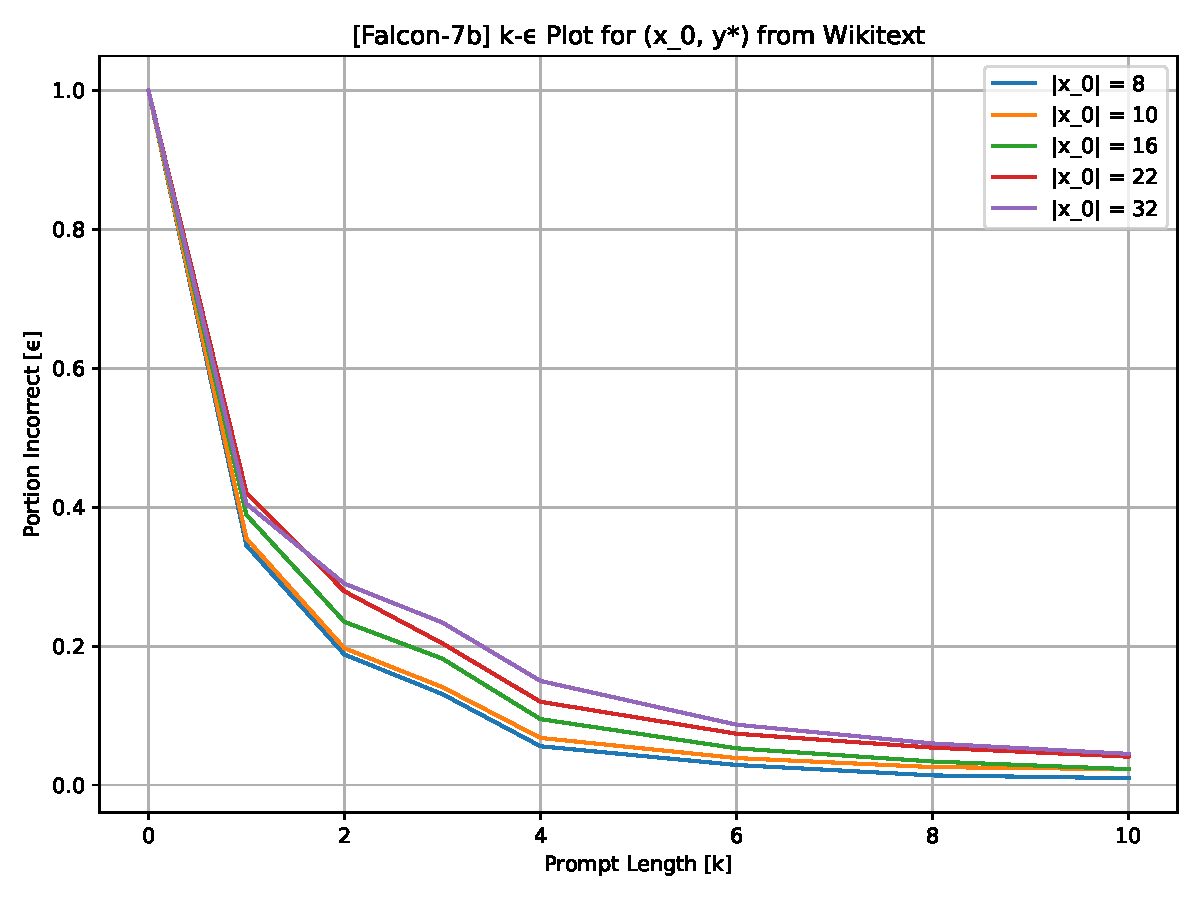
\includegraphics[width=\textwidth]{figs/og_falcon7b_k_epsilon.pdf}
    \end{minipage}
    \hfill
    % Second figure (on the right)
    \begin{minipage}[b]{0.48\textwidth}
        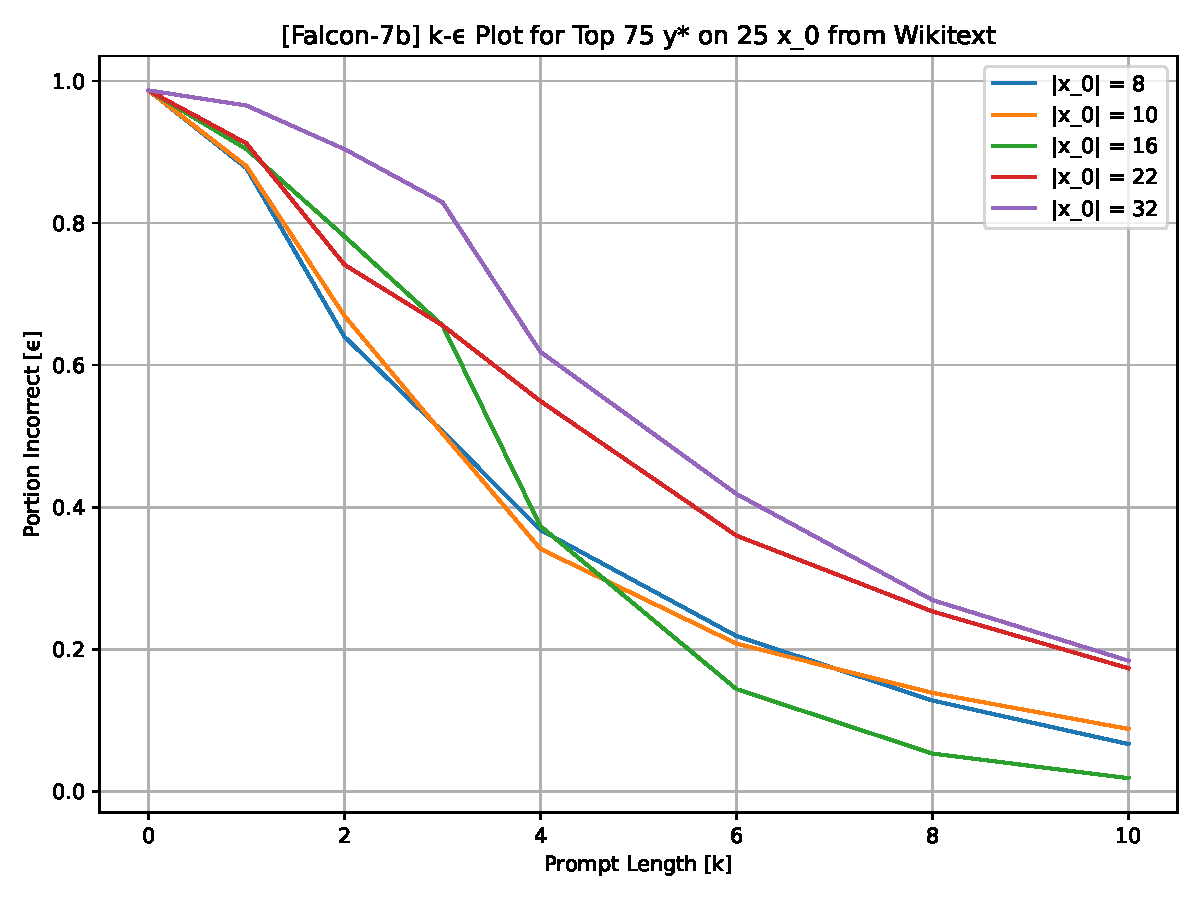
\includegraphics[width=\textwidth]{figs/shallow1_falcon7b_k_epsilon.pdf}
    \end{minipage}

    \vspace{1em} % Optional: add a bit of vertical space between the rows


    % Collective caption in the fourth quadrant
    \begin{minipage}[b]{0.48\textwidth}
        \caption{
            Main experimental results on $k-\epsilon$ controllability of Falcon-7b. \\
            \textbf{Top left}: $k-\epsilon$ values for Falcon-7b on ground truth target token $y^*$. 97.16\% of the instances were solved with a prompt of length $k\leq 10$. \label{fig:falcon_7b_k-e} \\
            \textbf{Top right}: $k-\epsilon$ values for reaching the top 75 most likely outputs $y^*$ for each $\mathbf x_0$. The top 75 targets were reachable at least 89.39\% of the time with a prompt of length $k\leq 10$.
            \label{fig:falcon_7b_top75} \\
            \textbf{Bottom right}: Prior likelihood rank of target token $y^*$ versus required prompt length to elicit $y^*$. Target tokens were sampled uniformly from the least to most likely token.
            \label{fig:deep_falcon_rank_k}
        }
    \end{minipage}
    \hfill
    % Third figure (below the second)
    \begin{minipage}[b]{0.48\textwidth}
        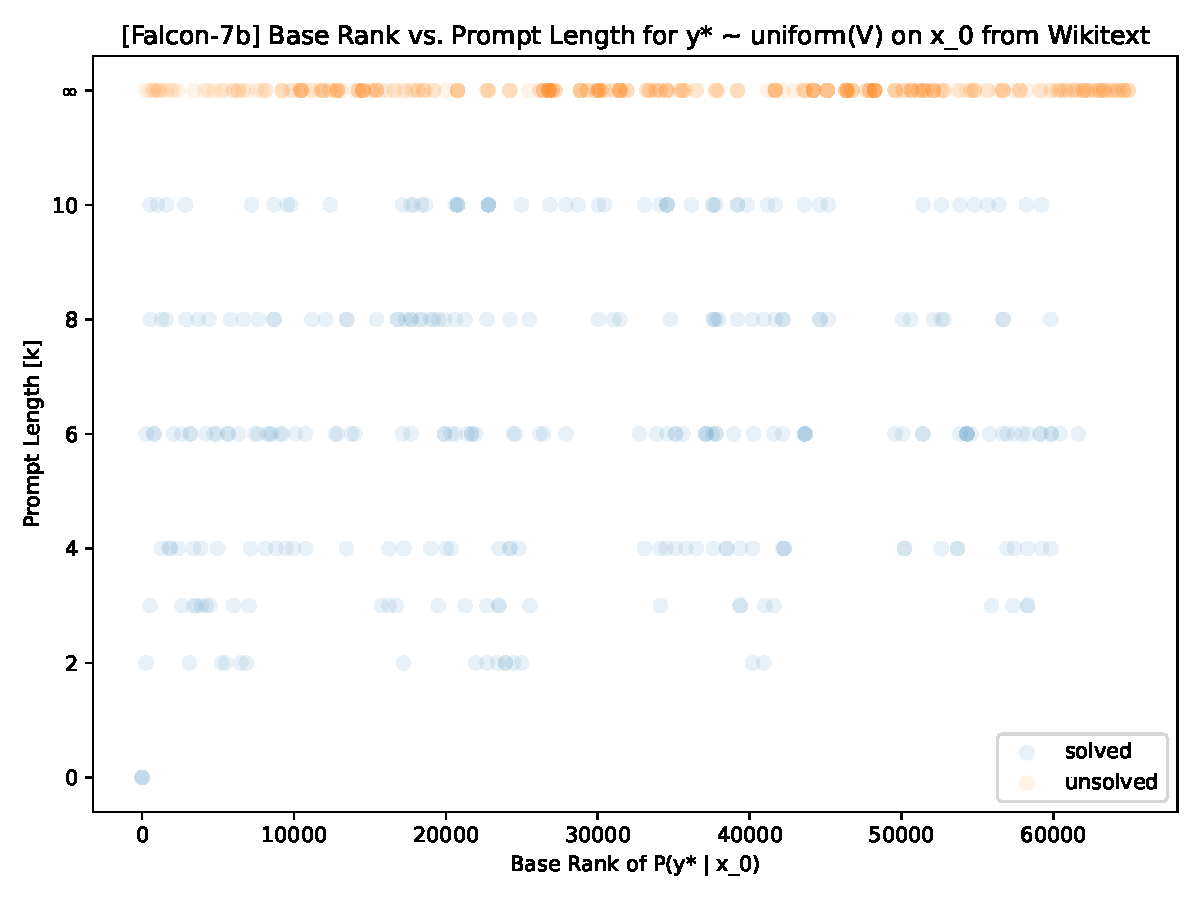
\includegraphics[width=\textwidth]{figs/deep1_falcon7b_base_rank_vs_prompt_length.pdf}
    \end{minipage}
\end{figure}


\paragraph{Top-75 reachability: } To explore the reachable set $R_y^k(\mathbf x_0)$ beyond the ground truth of Wikitext outputs, we generated a synthetic dataset of outputs by sampling 25 Wikitext sequences $\mathbf x_0$ and selecting the top 75 most likely next-tokens according to the model itself $P_{LM}(y | \mathbf x_0)$ as the target tokens (Figure~\ref{fig:falcon_7b_top75}, top right). We found that the top 75 output tokens were reachable over 85\% of the time for all models with control sequence length $k=10$. Supplementary figures including results for Llama-7b and Falcon-40b on $k-\epsilon$ controllability with respect to the top 75 most likely output tokens can be found in Section~\ref{sec:sup_75}.

\paragraph{Uniformly sampled target outputs: } To maximally push the bounds of the reachable set within our single output token scope, we created another synthetic dataset where the target output token $y^*$ was sampled uniformly from the highest likelihood next token to the lowest likelihood token. 
Although the overall $k-\epsilon$ score was relatively poor (only 46.43\% reachable with $k=10$ for Falcon-7b), we were intrigued by the near-uniform relationship between prior token rank (based on $P_{LM}(y | \mathbf x_0)$) versus the required number of prompt tokens. 
Figure~\ref{fig:deep_falcon_rank_k} (bottom right) plots the relationship between prior target token rank based on $P(y^* | \mathbf x_0)$ and the required prompt length $k$ to elicit the prompt. While over half were unreachable, the remaining reachable tokens appear uniformly distributed in terms of required prompt length, regardless of rank. Supplementary figures analyzing the $k-\epsilon$ controllability of Falcon-7b with respect to uniformly sampled target outputs $y$ can be found in Section~\ref{sec:sup_deep}. 

% Some example instances from Wiki-Text, with example prompts (greedy, various lengths, showing whether its correct or not).


\section{Discussion}
\label{sec:discussion}
% \label{sec:open_questions}

% 1: Re-iterate the results briefly
    % We proposed a control theoretic framework 
    % We demonstrated the existence of optimal prompts of length $k\leq 10$
    % We proved a bound on controllability of self-attention
We proposed a control theoretic framework for understanding language model prompting, orienting our investigation around the reachable set of outputs $\mathcal R_y^k(\mathbf x_0)$.
We proved a bound on the reachable set of outputs for self-attention in terms of the singular values of its weight matrices, and we established fundamental results on the reachability of ``correct'' next tokens (according to Wikitext). We expanded the scope of this investigation by probing the reachability of tokens assigned high likelihood by the LLM itself, and tokens assigned minimal likelihood by the LLM itself. 

Bounding the reachable set for self-attention is deeply related to the mechanism by which consistent representations are formed for multi-token generation.
Steering a language model to generate a desired token sequence requires that the control input induce a token representation in the right-most token such that the next token prediction logits $P(\mathbf y | \mathbf u + \mathbf x_0)$ achieves a desired value. 
Moreover, generated tokens are fed back into the model, and their representations must be steered as well to control iterated generation.
Self-attention is the primary mechanism by which the token representations exchange information, making the reachable set of output representations across multiple tokens in $\mathbf X_0$ for self-attention a fundamental part of LLM control theory. 


Our empirical results suggest that there is far more to the reachability of a given output than just prior likelihood or the prior rank the LLM assigns to a given token. 
Although prompt optimization-based $k-\epsilon$ controllability experiments are only able to provide a lower bound on the content of the reachable set, the ability to frequently control even the \textit{least likely} token to being the \textit{most likely} token with just a few input tokens is intriguing. 
We believe this result indicates the importance of further investigating the reachability and controllability of LLMs, particularly for developing capable and reliable LLM systems. 


Our investigations provide an entry into the understanding of LLM controllability via prompts. However, a comprehensive understanding necessitates extending our exploration into diverse regimes. 
Exploring the controllability with longer prompts and longer questions (base token sequences) will be pivotal. 
Equally important is the study of diverse models to verify the generality of our findings. %Our results indicate a similar level of controllability for the 40 billion parameter models as the 7 billion parameter models, with slightly less controllability for the large model. 
% On the other hand, we only tested the large model on 500 sequences rather than 5000 due to computational constraints. 
% Notably, the mean prompt length among solved Wikitext instances for Falcon-40b is 1.59 tokens, less than Falcon-7b (1.76 tokens) and Llama-7b (1.83 tokens). 
Moreover, the direct comparison of controllability scores of different model families is challenging since family uses a different tokenizer. The Llama family tokenizer, for instance, has a vocabulary of 30,000 tokens whereas the Falcon family has a vocabulary of 65,536 tokens. Further work is required to robustly compare controllability across models. 


An intriguing observation from our study is the log-linear relationship between prompt length $k$ and controllability fraction $\epsilon$ (see Figure~\ref{fig:log_main} in Appendix~\ref{sec:sup_figs}). 
While this is compelling within our studied domain, it raises the essential question: is this relationship robust outside our current explorative scope? 
Unearthing universal scaling laws in LLM controllability would not only inform practical control applications but also open the door for theoretical insight into the nature of LLM behavior.


The progress we have made, both in understanding the bounds on self-attention controllability and the empirical measures of $k-\epsilon$ LLM controllability, underscores the potential of this control theoretic framing for studying LLMs. 
Below is a non-exhaustive list of open problems in LLM control, all stemming from the framing in section~\ref{sec:definitions_ctrl}: 
\begin{itemize}
    \item \textbf{Control Properties of Chain-of-Thought:} Chain-of-Thought is a powerful technique where LLMs are allowed to generate intermediate tokens (i.e., ``thoughts'') between a question and an answer \citep{wei2023chainofthought}. 
    The control properties (e.g., stability, reachability) of systems leveraging these techniques are of great interest for understanding and composing systems of LLMs in the real world.  
    \item \textbf{Distributional Control:} To what extent can we control the output distribution of a language model $P_{LM}(\mathbf y | \mathbf x_0 + \mathbf u)$ to a desired distribution $P^*(\mathbf y)$?
    \item \textbf{Computational Cost of Control:} What are the performance characteristics of LLM control regularized by computational cost? 
    \item \textbf{Learnability of Control:} To what extent can LLMs learn to control each other? Work such as \cite{zhou2023large} showed that LLMs are capable of human-level prompt engineering, but it is unclear how well an LLM can learn to control another when explicitly optimized on the objective of LLM control. 
    %Proximal policy optimization and other fine-tuning approaches are of great interest for this task, as this would allow controller models to learn about the nature of prompt-based control, unlike \cite{zhou2023large} that only applies pre-trained models to generate alternative prompts. Our preliminary experiments on PPO for training control models indicated that LLMs are capable of improving at controlling other models beyond their pre-trained capacity, but the maximal extent of this improvement remains unclear.
    \item \textbf{Controllable Subspaces:} In the control of linear dynamical systems, it is known that uncontrollable systems are often coordinate transformable into a representation where a subset of the coordinates are controllable and a subset are uncontrollable \cite{control_bible}. We have shown that controllable and uncontrollable components naturally emerge for self-attention heads in section~\ref{sec:single_head} -- can this be generalized to transformer blocks with nonlinearities and residual streams? 
    \item \textbf{Composable LLM Systems:} One of the greatest boons of control theory is the ability to compose control modules and subsystems into an interpretable, predictable, and effective whole \citep{lian2002network}. 
    The composition of LLM systems (potentially with non-LLM control modules) is an exciting avenue for scaling super intelligent systems.
    % to maximally leverage the capabilities of LLMs. Depending on the aforementioned \textit{learnability of control}, collectives of LLMs may well learn to function in the same hyper-controllable regime demonstrated herein, enabling horizontal scaling of performance.
\end{itemize}



% \section{Conclusion}
% We formalized prompt engineering as an optimal control problem on LLMs and introduced a general framework for LLM systems and controllability. 
% In this framework, we define the $k-\epsilon$ controllability metric for measuring the steerability of LLMs with respect to an imposed text distribution. 
% After proving a bound on the controllability of self-attention in terms of the singular values of its weight matrices, we computed the $k-\epsilon$ controllability of a panel of models. 


% Surprisingly, we found that optimal control prompts (\textit{magic words}) of 10 tokens or less exist for over 97\% of the WikiText causal language modelling (CLM) instances surveyed. Each magic word, when prepended to the CLM instance, forces the model to predict the correct final token in the sequence. 
% Despite prior efforts on prompt optimization for improving LLM performance on zero-shot objectives, it was unknown until now exactly how controllable LLMs are via prompting. Our results indicate that the behavior of LLMs is not solely constrained by the weights of the model, but also by the sophistication of the prompt. 
% We find the control theoretic framework for analyzing LLMs fruitful both for addressing practical issues with prompting and for generating fundamental insights and useful lines of inquiry as to the nature of these models. 


% \subsubsection*{Author Contributions}
% If you'd like to, you may include  a section for author contributions as is done
% in many journals. This is optional and at the discretion of the authors.

% \subsubsection*{Acknowledgments}



\bibliography{bhargava}
\bibliographystyle{iclr2024_conference}

\newpage
\appendix

\newpage
\section{Abstract Systems and Control Theory Background}
\label{sec:definitions_ctrl}

This section aims to provide an overview of fundamental control-theoretic concepts from an abstract perspective. We primarily draw from \cite{control_bible, kalman1969topics}, and \cite{ogata2010modern}.

% [Definition of abstract system]
Diverse definitions of ``system'' or ``machine'' exist in the literature, all representing the same core concept but varying in mathematical details. We offer the following high-level definition based on \cite{control_bible}: 

\begin{definition}[System] \label{def:system}
A ``system'' or ``machine'' $\Sigma = (\mathcal{T, X, U}, \phi)$ consists of: 
\begin{itemize}
    \item $\mathcal T:$ The \textbf{time set} along which system state evolves. 
    \item $\mathcal X: $ The \textbf{state space}.
    \item $\mathcal U:$ The \textbf{input space}.
    \item $\phi: \mathcal{X \times U \times T}^2 \to \mathcal X: $ The \textbf{transition map}. 
\end{itemize}
A system may also be equipped with an output space and readout map $(\mathcal Y, h)$: 
\begin{itemize}
    \item $\mathcal Y:$ The \textbf{output space}. 
    \item $h: \mathcal{X \times U \times T}\to \mathcal Y: $ The \textbf{readout map}.
\end{itemize}
\end{definition}
In other words, at time $t\in \mathcal T$, the system's state takes on values $x \in \mathcal X$, and the control input takes values $u \in \mathcal U$. The system evolves over time with the transition map $\phi(x, u, t, t')$ that returns the new state value $x'\in \mathcal X$ at time $t'>t$. A system can also have a readout map $h(x, u, t)$ that produces the output value $y\in \mathcal Y$ given the current time, state, and input value. An input $u\in \mathcal U$ defined over interval $[t, t']$ may be said to \textit{steer the system} $\Sigma = (\mathcal{T, X, U}, \phi)$ from state $x_0$ to state $x'$ if $x' = \phi(x_0, u, t, t')$. A wide variety of systems are expressible within this framework. E.g., we obtain discrete-time dynamical systems for $\mathcal T = \mathbb Z^+$. Continuous-time dynamical systems emerge for $\mathcal T = \mathbb R^+$. 

Note that we assume that the system $\Sigma$ is time-invariant; its dynamics $\phi$ do not change as a function of time. This assumption is widely applicable and is often made in the literature \citep{kalman1969topics, ogata2010modern, control_bible} to simplify definitions and discussions of systems. 


Reachability is a core control theory concept and central to defining controllability. At their core, definitions of reachability revolve around the existence of control inputs $u\in \mathcal U$ that steer the system from a starting state $x_0 \in \mathcal X$ to some desired state(s). Following from \cite{kalman1969topics, control_bible}, we define state reachability as: 

\begin{definition}[State Reachability]
\label{def:state-reachability}
State $x \in \mathcal X$ is reachable from initial state $x_0\in \mathcal X$ for system $\Sigma=(\mathcal{T, X, U}, \phi)$ iff there exists some time $T$ and control input $u^* \in \mathcal U$ such that $u^*$ steers the system from state $x_0$ to state $x$ at time $T$.
\end{definition}

We may use this definition of state reachability to define the reachable state set for some initial state $x_0 \in \mathcal X$:

\begin{definition}[Reachable State Set]
\label{def:reachable-state-set} 
The reachable state set from initial state $x_0 \in \mathcal X$ for system $\Sigma = (\mathcal {T, X, U}, \phi)$ is denoted $\mathcal R(x_0) \subseteq \mathcal X$ and consists of all reachable states $x\in \mathcal X$ from initial state $x_0$ (cf. Definition~\ref{def:state-reachability}). 
\end{definition} 


For systems with readout maps $h$, notions of \textit{output reachability} arise naturally. Note that state reachability is neither necessary nor sufficient to guarantee output reachability. 

\begin{definition}[Output Reachability]
\label{def:output-reachability}
Output $y \in \mathcal Y$ is reachable from initial state $x_0 \in \mathcal X$ for system $\Sigma=(\mathcal{T, X, U}, \phi, \mathcal Y, h)$ iff there exists some time $T$ and control input $u^* \in \mathcal U$ such that $u^*$ steers the system from state $x_0$ to output $y$ in time $T$. 
\end{definition}

\begin{definition}[Reachable Output Set]
\label{def:reachable-output-set}
The reachable output set from initial state $x_0 \in \mathcal X$ for system $\Sigma = (\mathcal{T, X, U}, \phi, \mathcal Y, h)$ is denoted $\mathcal R_y(x_0)$ and consists of all reachable outputs $y\in \mathcal Y$ from initial state $x_0$ (cf. Definition~\ref{def:output-reachability}). 
\end{definition}




A system is controllable when the reachable set extends to the entire state space. Practically speaking, this implies that one can steer the system from any initial state to any desired state. 

\begin{definition}[State Controllability]
\label{def:state-controllability} 
System $\Sigma = (\mathcal{T, X, U}, \phi)$ is state controllable iff, for every initial state $x_0\in \mathcal X$, the reachable set $\mathcal R(x_0) = \mathcal X$.
\end{definition}

\begin{definition}[Output Controllability] 
\label{def:output-controllability}
System $\Sigma = (\mathcal{T, X, U}, \phi, \mathcal Y, h)$ is output controllable iff, for every initial state $x_0\in \mathcal X$, the reachable output set $\mathcal R_y(x_0) = \mathcal Y$.
\end{definition}


A range of fruitful questions stem from these definitions: if there is a cost associated with control inputs $u\in \mathcal U$ (e.g., power constraints, length constraints), what is the minimum cost of control? What is the minimum time required to get from the initial state to the desired final state or output? If the system is not completely controllable, under what conditions is it controllable? Under which readout maps is a system output controllable? 















\newpage
\section{Proof of Self-Attention Controllability Theorem~\ref{thm:attention-control}}
\label{app:proof-control-llms}
\textit{Note: Key terms for the proof are introduced in Section~\ref{sec:single_head} surrounding Theorem~\ref{thm:attention-control}. Specifically, the definition of self-attention mechanism $\Xi$, the control problem setup, and the reachable set $\mathcal R_y^k(\mathbf X_0)$ are required background for this proof.}

\begin{proof}
    For each token representation matrix $\mathbf{Q, K, V} \in \mathbb R^{(k+M) \times \cdot}$, we denote the first $k$ rows corresponding to $\mathbf U$ using $u$ as a subscript, like $\mathbf Q_u$. The remaining $M$ rows corresponding to $\mathbf X_0$ are denoted with subscript $x$ like $\mathbf Q_x$. 
    
    Let $\mathbf A$ be the exponentiated query-key outer product matrix with the following block structure: 
    \begin{equation}
        \label{eqn:def-A}
        \mathbf A = \exp \begin{pmatrix}
            \frac{
                \textbf{Q K}^\top
            }{
                \sqrt{d_k}
            }
        \end{pmatrix}
        = \exp \begin{pmatrix} 
            \begin{bmatrix}
                \mathbf{Q_u K_u^\top} & \mathbf{Q_u K_x^\top} \\
                \mathbf{Q_x K_u^\top} & \mathbf{Q_x K_x^\top}
            \end{bmatrix}
            \frac{1}{\sqrt{d_k}}
        \end{pmatrix}
         = \begin{bmatrix}
             \mathbf A_{uu} & \mathbf A_{ux} \\ 
             \mathbf A_{xu} & \mathbf A_{xx} 
         \end{bmatrix}
    \end{equation}

    We apply a similar quadrant decomposition to $\mathbb D$, defined initially in Equation~\ref{eqn:denominator-definition}.
    \begin{equation}
        \label{eqn:denom-decomp}
        \mathbb D = \text{diag}\begin{pmatrix} \exp\begin{pmatrix} \frac{\mathbf{QK}^\top}{\sqrt{d_k}} \end{pmatrix} \mathbf 1_{N\times 1} \end{pmatrix}
        = \begin{bmatrix}
            \mathbb D_u & \mathbf 0 \\ 
            \mathbf 0 & \mathbb D_x \\ 
        \end{bmatrix}
    \end{equation}

    where the quadrant demarcations in $\mathbb D$ follow from Equation~\ref{eqn:def-A}. 

    We may now express the self-attention mechanism output representations $\mathbf Y$ as 
    \begin{equation}
        \label{eqn:y-decomp}
        \mathbf Y = \mathbb D_x^{-1} \mathbf A_{xu} \mathbf V_u + \mathbb D_x^{-1} \mathbf A_{xx} \mathbf V_x
    \end{equation}

     

    We begin by stating the equality between the desired output $\mathbf Y^*$ and the true system output from Equation~\ref{eqn:y-decomp}. The final bound in Equation~\ref{eqn:attention-reachability-condition} of Theorem~\ref{thm:attention-control} is derived by isolating terms depending on control input $\mathbf U$, bounding them, and expressing that bound as a condition for achieving equality between the desired output $\mathbf Y^*$ and the true system output.
    \begin{align}
        \label{eqn:init-equality}
        \mathbf Y^* &= 
        \underbrace{
            \mathbb D_x^{-1} \mathbf A_{xu} \mathbf V_u
        }_{
            \triangleq \mathbf Y_u
        }+ 
        \underbrace{
            \mathbb D_x^{-1} \mathbf A_{xx} \mathbf V_x 
        }_{
            \triangleq \mathbf Y_x
        } \\ 
        \implies \mathbf Y_u &= \mathbf Y^* - \mathbf Y_x
    \end{align}


    We may immediately bound the magnitude of the rows of $\mathbf Y_u$ as the matrix $\mathbb D_x^{-1} \mathbf A_{x_u}$ has rows that sum to less than 1 (it represents one quadrant of the row-wise softmaxed attention map, which has rows that sum to 1 by construction). 
    Therefore, each row $\mathbf y_u^i$ of $\mathbf Y_u$ lies within the convex hull defined by the row vectors $\mathbf v_u^i$ of $\mathbf V_u$. 
    Recalling Definition~\ref{def:self-attention}, $\mathbf V_u = \mathbf {U W_v}$. Let $\Omega_u = \max_j \|\mathbf u^j\|$ for rows $\mathbf u^j$ of $\mathbf U$, we can bound the norm of each $\mathbf v_u^i$ in $\mathbf V_u$ with the maximum singular value of parameter matrix $\mathbf W_v$, denoted $\sigma_q$. 
    Refer to Chapter 5 of \cite{367_optimization_models} for an overview of singular values. 
    Thus we may bound each $\| \mathbf v_u^i \| \leq \Omega_u \sigma_q$. By the properties of convex hulls, each row of $\mathbf Y_u$ must inherit this upper bound on magnitude to retain feasibility.
    \begin{equation}
        \label{eqn:y_u_bound}
        \| \mathbf y_u^i \| < \Omega_u \sigma_q 
    \end{equation}
    Refer to Chapter 8 of \cite{367_optimization_models}) for a detailed explanation of convex hulls and their properties. 

    While $\mathbf Y_x$ in Equation~\ref{eqn:init-equality} may appear to depend only on imposed $\mathbf X_0$, the denominator term $\mathbb D_x^{-1}$ contains influences from $\mathbb U$. Let us split the denominator term $\mathbb D_x = \hat{\mathbf D}_{xx} + \hat{\mathbf D}_{xu}$ where $\hat{\mathbf D}_{xx}$ depends solely on the imposed input $\mathbb X_0$. $\hat{\mathbf D}_{xx}$ is definedin Equation~\ref{eqn:dxx}. Let $\hat{\mathbf D}_{xu}$ be defined as: 
    \begin{align}
        \label{eqn:Dxu-definition}
        \hat{\mathbf D}_{xu} &= \text{diag}\begin{pmatrix}
            \exp\begin{pmatrix}
                \frac{\mathbf{Q_x K_u}^\top}{\sqrt{d_k}}
            \end{pmatrix}
            \mathbf 1_{k \times 1}
        \end{pmatrix} 
    \end{align}

    Recall Equation~\ref{eqn:hat-Y_x-def}, which defines $\hat{\mathbf Y}_x$, the output of $\Xi$ if only $\mathbf X_0$ is input. 
    Let us express the condition in Equation~\ref{eqn:init-equality} using $\hat{\mathbf Y}_x$ to disentangle the influence of the control input: 

    \begin{equation}
        \mathbf Y_u = \mathbf Y^* - (\hat{\mathbf D}_{xu} + \hat{\mathbf D}_{xx})^{-1} \hat{\mathbf D}_{xx} \hat{\mathbf Y}_x
    \end{equation}

    Observe that the rows of $\mathbf Y_x$ and $\hat{\mathbf Y}_x$ are positively scaled versions of each other because the denominator matrices are all positive and diagonal. 
    Applying the bound in Equation~\ref{eqn:y_u_bound} using row-wise notation, 

    \begin{align}
        \label{eqn:almost_done}
        \| {\mathbf y^*}^i - \frac{
            \hat D_{xx}^i
        }{
            \hat D_{xx}^i + \hat D_{xu}^i
        }
        \hat{\mathbf y}_x^i \| 
        \leq 
        \sigma_q \Omega_u
    \end{align}

    Using the same singular values reasoning as in Equation~\ref{eqn:y_u_bound} to bound the unknown denominator term $\hat D^i_{xu}$, which is the only term still dependent on the control input $U$. 

    \begin{equation}
        \hat D_{xu}^i \leq k \exp \begin{pmatrix}
            \frac{\Omega_x \sigma_q \sigma_k \Omega_u}{\sqrt{d_k}}
        \end{pmatrix}
    \end{equation}

    Achieving this minimum value will minimize the value of $\mathbf y_x^i$ by maximally scaling down $\hat{\mathbf y}_x^i$. 
    The maximum value for $\mathbf y_x^i$ arises when $\hat{D}_{xu}^i$ is minimized (e.g., to zero) resulting in $\mathbf y_x^i = \hat{\mathbf y_x^i}$. 

    Therefore, the the value of $\mathbf y_x^i$ is constrained linear scalings between this minimum and this maximum. 
    If every scaling violates the inequality in Equation~\ref{eqn:almost_done}, then the system is strictly controllable. 

    Therefore, if $\langle {\mathbf y^*}^i, \hat {\mathbf y}_x^i  \rangle \leq 0$ for some row $i$ 
    following inequality is met, the output $Y^*$ is \textbf{strictly unreachable} under imposed input representations $\mathbf X_0$ and control input $\mathbf U$: 

    \begin{align}
        \label{eqn:finale}
        \| {\mathbf y^*}^i - \frac{
            \hat D_{xx}^i
        }{
            \hat D_{xx}^i + k \exp \begin{pmatrix}
            \frac{\Omega_x \sigma_q \sigma_k \Omega_u}{\sqrt{d_k}}
        \end{pmatrix}
        }
        \hat{\mathbf y}_x^i \| 
        \leq 
        \sigma_q \Omega_u
    \end{align}

    % To continue isolating controllable versus uncontrollable terms from Equation~\ref{eqn:init-equality}, observe that $\mathbf Y^*$ is imposed (known), and $\mathbf Y_x$ is a function of primarily imposed $X_0$, except for the denominator matrix $\mathbb D_x^{-1}$, which depends on both $\mathbf X_0$ and $\mathbf U$.  

    % To disentangle the influence of control input representation $\mathbf U$ and imposed state representation $\mathbf X_0$, we introduce disentangled $\hat{\mathbf Y}_x$, which represents the output of $\Xi$ if only the imposed state representation $\mathbf X_0$ were input. 
    % We can relate $\mathbf Y_x$ and $\hat{\mathbf Y}_x$ via the partial denominator matrix $\hat{\mathbf D}_{xx}$ defined in Equation~\ref{eqn:dxx} as follows: 

    % \begin{align}
    %     \label{eqn:y_x-hat-identity}
    %     \hat{\mathbf Y}_x &= \mathbb D_x \hat{\mathbf D}_{xx}^{-1}  \\
    %     \mathbf Y_x &= \mathbb D_x^{-1} \hat{\mathbf D}_{xx} \hat{\mathbf Y}
    % \end{align}

    % We also introduce diagonal matrix $\hat{\mathbf D}_{xu}$ similar to $\hat{\mathbf D}_{xx}$: 
    % \begin{align}
    %     \label{eqn:Dxu-definition}
    %     \hat{\mathbf D}_{xu} &= \text{diag}\begin{pmatrix}
    %         \exp\begin{pmatrix}
    %             \frac{\mathbf{Q_x K_u}^\top}{\sqrt{d_k}}
    %         \end{pmatrix}
    %         \mathbf 1_{k \times 1}
    %     \end{pmatrix} \\
    % \implies \mathbb D_x &= \hat{\mathbf D}_{xu} + \hat{\mathbf D}_{xx}
    % \end{align}

    % Thus we may express the attention denominator matrix $\mathbb D_x$ in two components: $\hat{\mathbf D}_{xx}$, which is independent of control input $\mathbf U$, and $\hat{\mathbf D}_{xu}$, which is dependent on control input $\mathbf U$. 
    % We may also bound the entries along the diagonal in $\hat{\mathbf D}_{xu}$ given in Equation~\ref{eqn:Dxu-definition}

    % \begin{align}
    %     \label{eqn:Dxu-bound}
    %     \exp\begin{pmatrix}
    %         \frac{
    %             \mathbf{Q_x K_u}^\top
    %         }{\sqrt{d_k}}
    %     \end{pmatrix} \mathbf 1_{k\times 1}
    %     \leq 
    %     k \exp \begin{pmatrix}
    %         \frac{\Omega_x \sigma_q \sigma_k \Omega_u}{\sqrt{d_k}}
    %     \end{pmatrix}
    % \end{align}

    % Continuing from Equation~\ref{eqn:init-equality}, 
    % \begin{align}
    %     \mathbf Y_u &= \mathbf Y^* - \mathbf Y_x \\
    %     &= \mathbf Y^* - \mathbb D_x^{-1} \hat{\mathbf D}_{xx} \hat{\mathbf Y}_x \\ 
    %     \mathbf Y_u &= \mathbf Y^* - (\hat{\mathbf D}_{xu} + \hat{\mathbf D}_{xx})^{-1} \hat{\mathbf D}_{xx} \hat{\mathbf Y}_x
    % \end{align}

    % Observe that $\hat{\mathbf D}_{xu}$ appears under an inverse operator, and every element of its diagonal is bounded from above by Equation~\ref{eqn:Dxu-bound}, suggesting that its inverse can be bounded from below. 
    % Recall that the lefthand side $\mathbf Y_u$ also has an element-wise bound from below. 
    % This is made clearer in the row-wise picture using notation introduced for Equation~\ref{eqn:attention-reachability-condition} in Theorem~\ref{thm:attention-control}: 

    % \begin{align}
    %     \mathbf y_u^i  &= 
    %         \mathbf {y^*}^i 
    %         - \frac{
    %             \hat D_{xx}^i
    %         }{
    %             \hat D_{xx}^i 
    %             + \hat D_{xu}^i
    %         }
    %         \hat{\mathbf y}_x^i \\
    %     \implies 
    %     \|\mathbf y_u^i \| &= 
    %         \| 
    %             \mathbf {y^*}^i 
    %             - \frac{
    %                 \hat D_{xx}^i
    %             }{
    %                 \hat D_{xx}^i 
    %                 + \hat D_{xu}^i
    %             }
    %             \hat{\mathbf y}_x^i
    %         \| \\ 
    %     &\leq \| \mathbf {y^*}^i \| + 
    %         \|
    %             \frac{
    %                     \hat D_{xx}^i
    %             }{
    %                 \hat D_{xx}^i 
    %                 + \hat D_{xu}^i
    %             }
    %             \hat{\mathbf y}_x^i
    %         \| \\
    %     &\geq \| \mathbf {y^*}^i \| + 
    %         \frac{
    %                 \hat D_{xx}^i
    %         }{
    %             \hat D_{xx}^i 
    %             + 
                % k \exp \begin{pmatrix}
                %     \frac{\Omega_x \sigma_q \sigma_k \Omega_u}{\sqrt{d_k}}
                % \end{pmatrix}
    %         }
    %         \| \hat{\mathbf y}_x^i \|
    % \end{align}
    

\end{proof}












\newpage
\section{Prompt Optimization Algorithms}
\label{sec:algs}

\paragraph{Greedy Back-Generation: } While testing all prompts in $\mathcal V^k$ is intractable for $k >1$, it takes only $|\mathcal V|$ forward passes of the network to compute the loss on $y$ induced by all possible \textit{single token} prompts $u \in \mathcal V$. Our Greedy Back Generation algorithm leverages this fact to generate prompts $u\in \mathcal V^k$ one token at a time, working backward sampling the $i$th greedy-optimal single token extension $u' = \arg\max_{u'} P_{LM}(y|u'+u+x)$ of the current prompt $u\in \mathcal V^{i-1}$. 

\begin{algorithm}
\label{alg:greedy}
\caption{Greedy Token-Wise Prompt Generation}
\begin{algorithmic}[1]
\Require A causal LLM $P_{LM}$ with vocabulary $\mathcal V$, a set of base tokens $x \in \mathcal V^n$, a desired final token $y\in \mathcal V$, and a desired number of prompt tokens $k$.
\Ensure \textit{Magic words} $u^*$ of length $k$.
\State Initialize $u^*$ to be empty.
\For{$i$ from $1$ to $k$}
    \ForAll{$u' \in \mathcal V$}
        \State compute $P_{LM} (y | u'+u^*+x)$
    \EndFor
    \State Select the $u'$ that maximizes the probability of $y$ given $u' + u^* + x$. Prepend $u'$ to $u^*$
\EndFor
\State \Return $u^*$
\end{algorithmic}
\end{algorithm}
This method is optimal for $k=1$ prompt token $u^{*}\in \mathcal V$ and generally outperforms GCG for short prompts of length $k\leq 3$. Computing 1 additional prompt token takes roughly 1-4 minute when using an NVIDIA A100-80GB GPU with a 7 billion parameter model and 5-20 minutes on 2 NVIDIA A100-80GB GPUs with a 40 billion parameter model. 




% Greedy coordinate gradient (SoTA) 
\paragraph{Greedy Coordinate Gradient (GCG): } The Greedy Coordinate Gradient algorithm, presented by \citep{zou2023universal} building off the work of \citep{shin2020autoprompt}, is the state-of-the-art method for optimizing prompts. Starting with a random prompt of length $k$, the algorithm generates a batch of alternative prompts. Each member of the batch swaps a random token in the current prompt with a promising alternate token. The value metric for a swap is given by a first order approximation of the change in loss $\mathcal L = \text{CELoss}(y, P_{LM}(y | u + x))$ with the embedding of each token in $u$. 

\begin{algorithm}
\label{alg:gcg}
\caption{Greedy Coordinate Gradient}
\begin{algorithmic}[1]
\Require A causal LLM $P_{LM}$ that accepts token strings from a vocabulary $\mathcal X$, an embedding dictionary $\mathbf{e}$, embeddings $\mathbf{e}^{*}_i$ corresoponding to each token $i$ of $u^*$, a set of base tokens $x_{1:n}$, a desired number of prompt tokens $k$, iterations $T$, $k_{sub}$, and batch size $B$.
\Ensure \textit{Magic words} $u^*$ of length $k$.
\State Initialize $u^*$ to be random tokens from vocabulary.
\For{$iteration$ from $1$ to $T$}
    \For{$i$ from $1$ to $k$}
        \Comment{Compute the top $k_{sub}$ most promising substitutions.}
        \State $\mathcal X_i = $ Top-$k_{sub} (\mathbf{e}^T \nabla_{\mathbf{e}^{*}_i} P_{LM}(x_n | u^* + x_{1:n-1}))$ \label{line:cand_calc}
    \EndFor
    \For{$b$ from $1$ to $B$} \label{line:for_batch}
        \State $i = $ randint([1, \dots, $k$])
        \Comment{Select random position to swap.}
        \State $j = $ randint([1, \dots, $k_{sub}$]
        \Comment{Select random token from candidate set.}
        \State $\tilde{u}^{*}_b [i] = \mathcal X_i [j]$ 
        \Comment{Swap token at position $i$.}
    \EndFor
    \State $u^{*} = \tilde{u}^{*}_{b^\ast}$ , where $b^\ast = $ argmax$_b (P_{LM}(x_n | u^* + x_{1:n-1})))$
    \Comment{Select replacement which maximizes probability of future token.}
\EndFor
\State \Return $u^*$
\end{algorithmic}
\end{algorithm}

This method outperforms all other methods we tested for prompts of length $k>3$. We use a batch size $B=768$, sampled from the top $k_{sub}=128$ token replacements at each index, and iterate for $T=34$ iterations. 
For each instance, this optimization took roughly 2 minutes for the 7 billion parameter models on a single A100-80GB GPU and 4-8 minutes for the 40 billion parameter model on 4 A100-80GB GPU.






\newpage
\section{Supplementary Figures: Optimal Control Prompts}
\label{sec:sup_figs}

\subsection{``Ground Truth'' Controllability Results}
\label{sec:sup_main}
This subsection includes supplementary figures for the controllability of Llama-7b, Falcon-7b, and Falcon-40b ``ground truth'' target outputs from Wikitext. For each initial state sequence $\mathbf x_0$, the target output $y$ is the token immediately following $\mathbf x_0$ in Wikitext. 
We measured the $k-\epsilon$ controllability of each of the 7 billion parameter models with a dataset of 5000 state-output pairs while we used a dataset of 500 state-output pairs for Falcon-40b. 

Figure~\ref{fig:log_main} shows each model's log-spaced $k-\epsilon$ curves on the Wikitext dataset, revealing a log-linear relationship between maximum prompt length $k$ and the fraction of uncontrollable initial state-target output pairs $(\mathbf x_0, y)$. 
We visualize the relationship between prompt length and the prior cross-entropy loss of each LLM on predicting the target output $y$ given the state sequence $\mathbf x_0$ (i.e., $-\log P_{LM}(y | \mathbf x_0)$ in Figure~\ref{fig:base_loss_k_main} where we find it difficult to predict the required prompt length from the base loss. 

Finally, Figure~\ref{fig:main_freqs} shows a histogram of the tokens in the optimized prompts generated in the ground truth $k-\epsilon$ controllability experiments on Wikitext. 

\begin{figure}[ht]
    \centering
    % First figure (on the left)
    \begin{minipage}[b]{0.48\textwidth}
        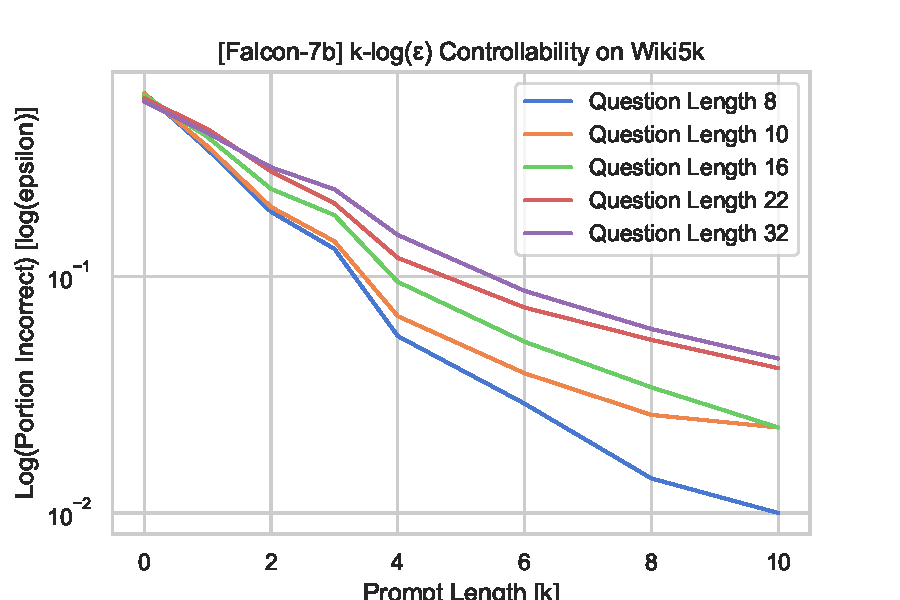
\includegraphics[width=\textwidth]{old_figs/falcon_7b/log_line_plot.pdf}
    \end{minipage}
    \hfill
    % Second figure (on the right)
    \begin{minipage}[b]{0.48\textwidth}
        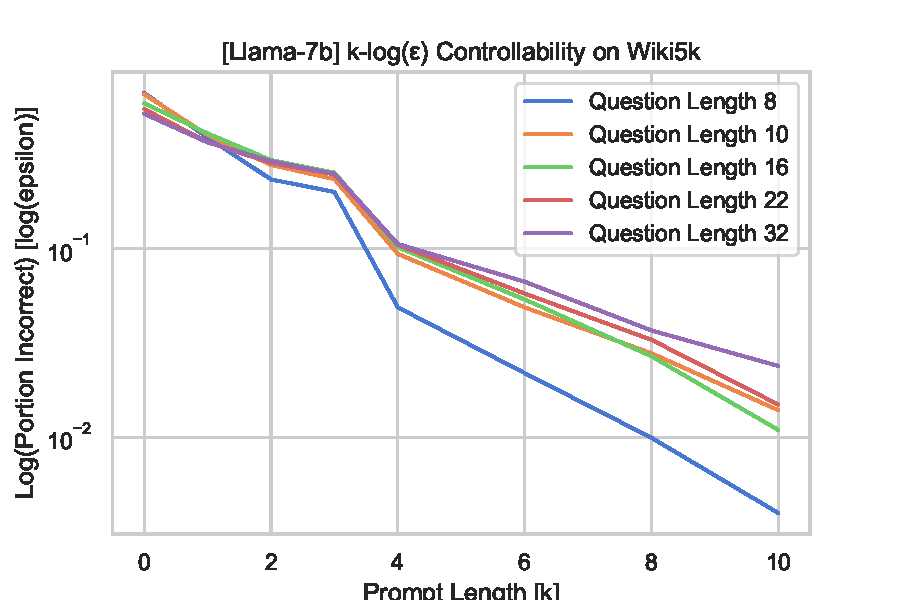
\includegraphics[width=\textwidth]{old_figs/llama_7b/log_line_plot.pdf}
    \end{minipage}
    \vspace{1em} % Optional: add a bit of vertical space between the rows
    % Collective caption in the fourth quadrant
    \begin{minipage}[b]{0.48\textwidth}
        \caption{
            Log spaced main results of $k-\log(\epsilon)$ controllability. Interestingly, the relationship between $k$ and $\log(\epsilon)$ appears roughly linear for each question length in the regime studied. \\
            \textbf{Top left}: $k-\log(\epsilon)$ values for Falcon-7b. With $k=10$ control tokens, 97.16\% of the target outputs were reachable. \\
            \textbf{Top right}: $k-\log(\epsilon)$ values for Llama-7b. With $k=10$ control tokens, 98.64\% of the target outputs were reachable. \\
            \textbf{Bottom right}: $k-\log(\epsilon)$ values for Falcon-40b. With $k=10$ control tokens, 97.00\% of the target outputs were reachable.
            \label{fig:log_main}
        }
    \end{minipage}
    \hfill
    % Third figure (below the second)
    \begin{minipage}[b]{0.48\textwidth}
        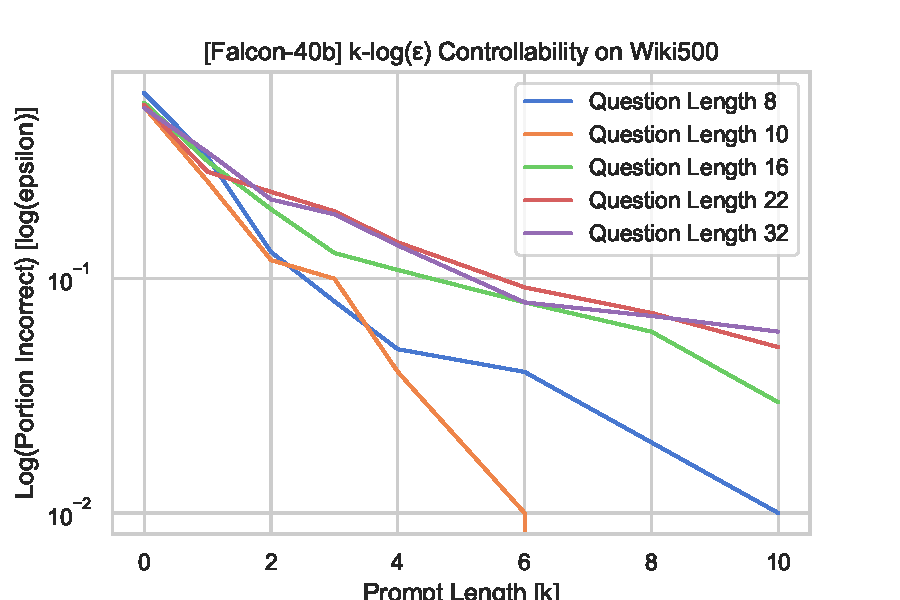
\includegraphics[width=\textwidth]{old_figs/falcon_40b/log_line_plot.pdf}
    \end{minipage}
\end{figure}

\begin{figure}[ht]
    \centering
    % First figure (on the left)
    \begin{minipage}[b]{0.48\textwidth}
        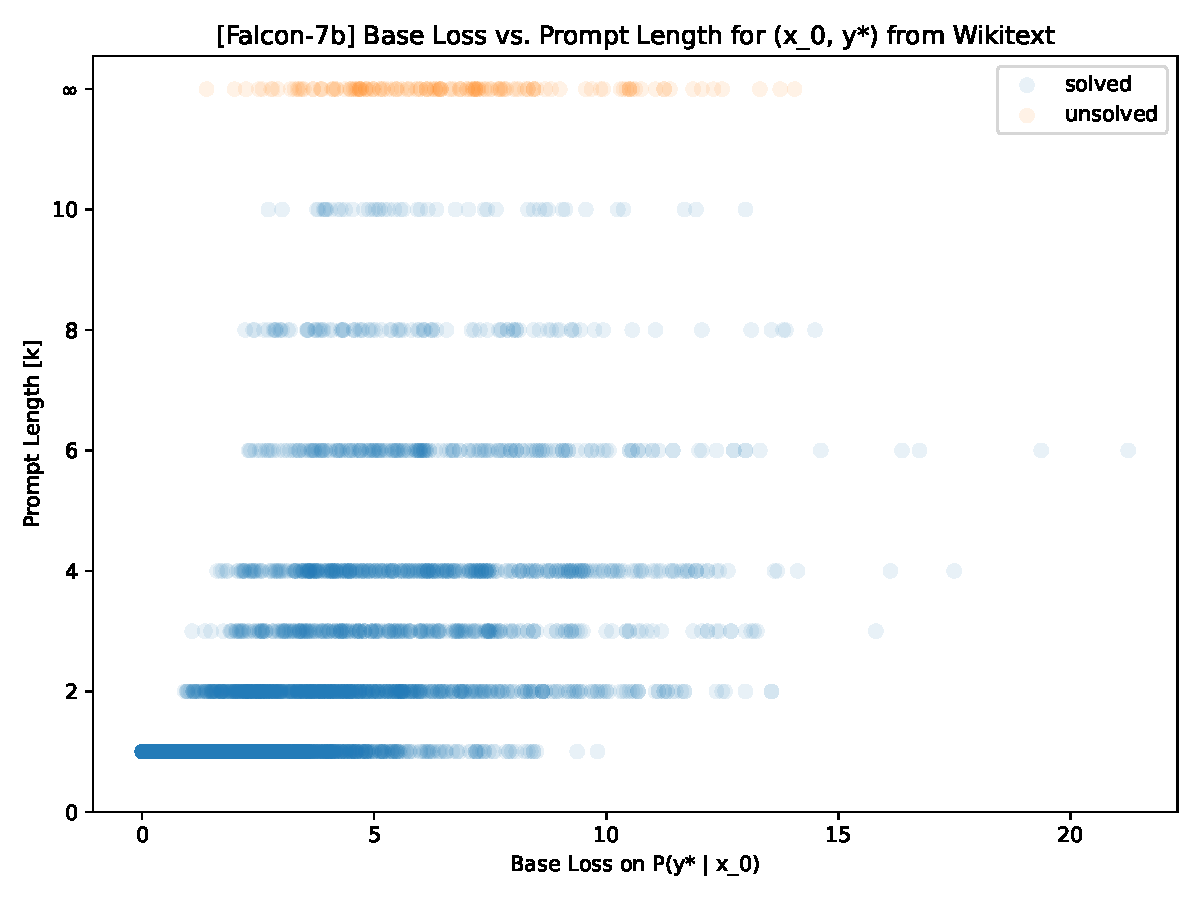
\includegraphics[width=\textwidth]{figs/og_falcon7b_base_loss_vs_prompt_length.pdf}
    \end{minipage}
    \hfill
    % Second figure (on the right)
    \begin{minipage}[b]{0.48\textwidth}
        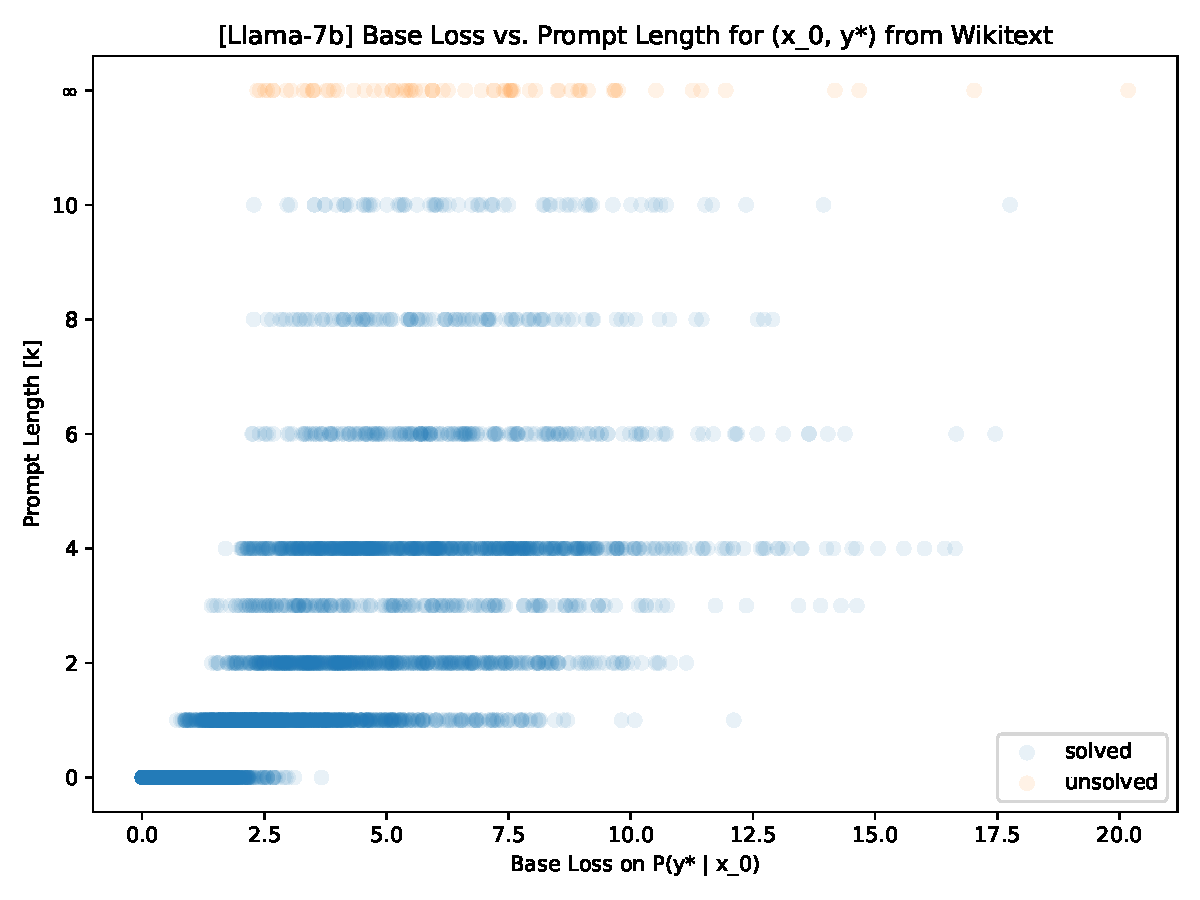
\includegraphics[width=\textwidth]{figs/og_llama7b_base_loss_vs_prompt_length.pdf}
    \end{minipage}
    
    \vspace{1em} % Optional: add a bit of vertical space between the rows
    
    
    % Collective caption in the fourth quadrant
    \begin{minipage}[b]{0.48\textwidth}
        \caption{
            Required prompt length $k$ versus base loss on the target output $\mathcal L = -\log P_{LM}(y | \mathbf x_0)$. 
            While there does appear to be an ``exclusion zone'' in the top left-hand corner where a high prompt length is never associated with a base loss below a given threshold, base loss appears to be a poor predictor of required prompt length.
            \label{fig:base_loss_k_main}
        }
    \end{minipage}
    \hfill
    % Third figure (below the second)
    \begin{minipage}[b]{0.48\textwidth}
        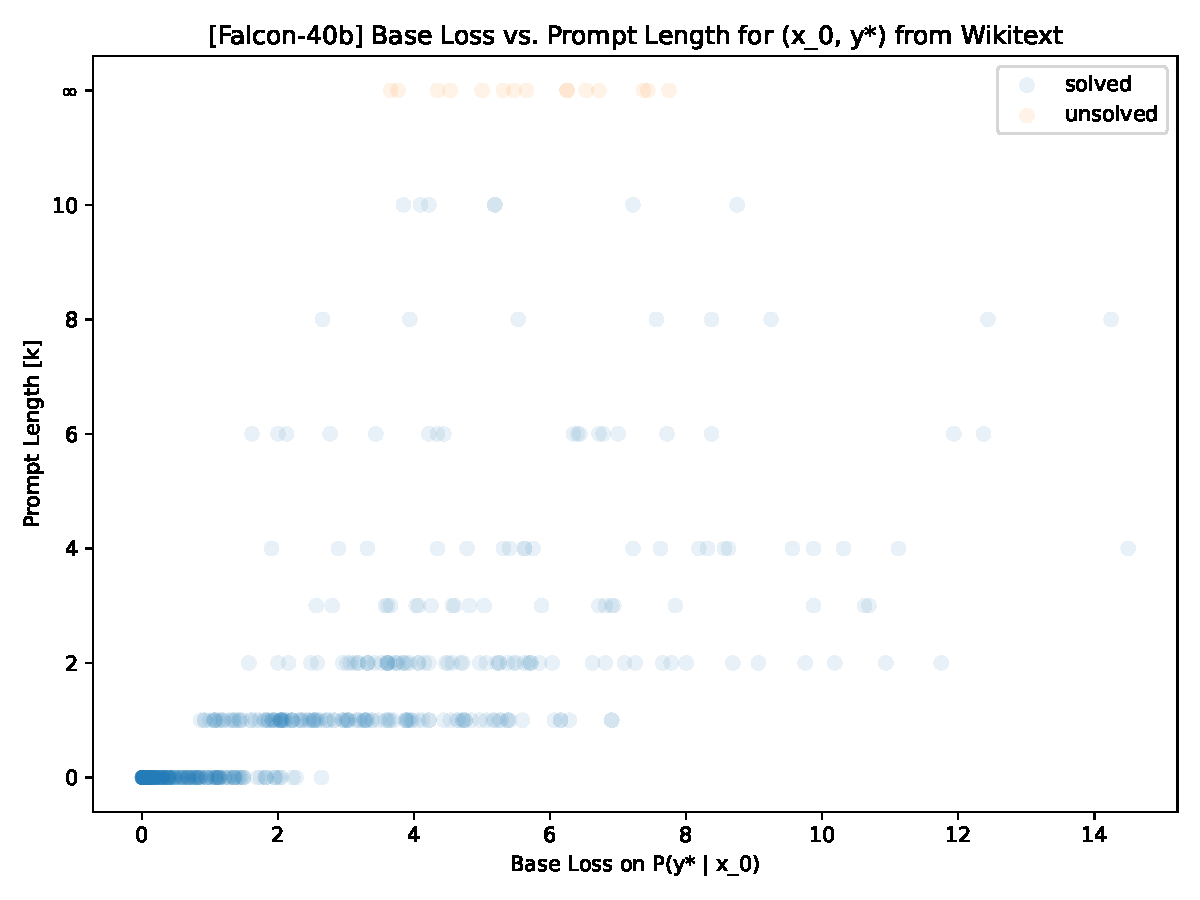
\includegraphics[width=\textwidth]{figs/og_falcon40b_base_loss_vs_prompt_length.pdf}
    \end{minipage}
\end{figure}


\begin{figure}[htbp]
    \centering
    \subfigure[Falcon-7b]{
        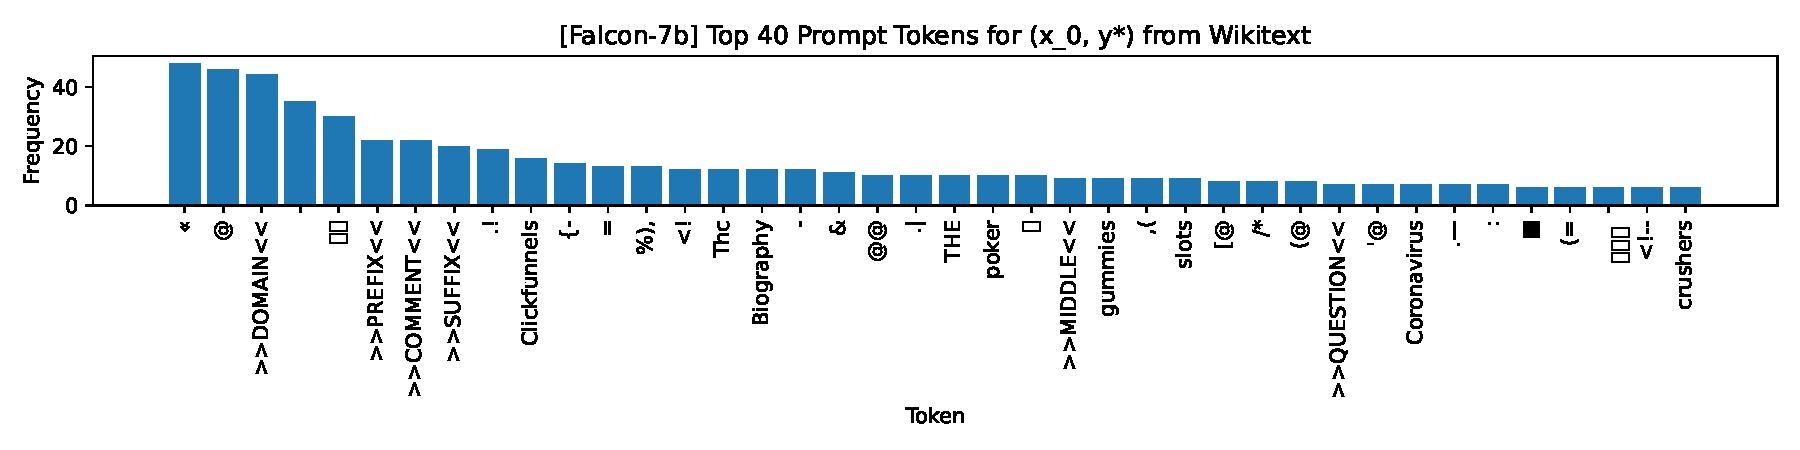
\includegraphics[width=0.9\textwidth]{figs/og_falcon7b_prompt_token_freqs.pdf}
    }
    \subfigure[Llama-7b]{
        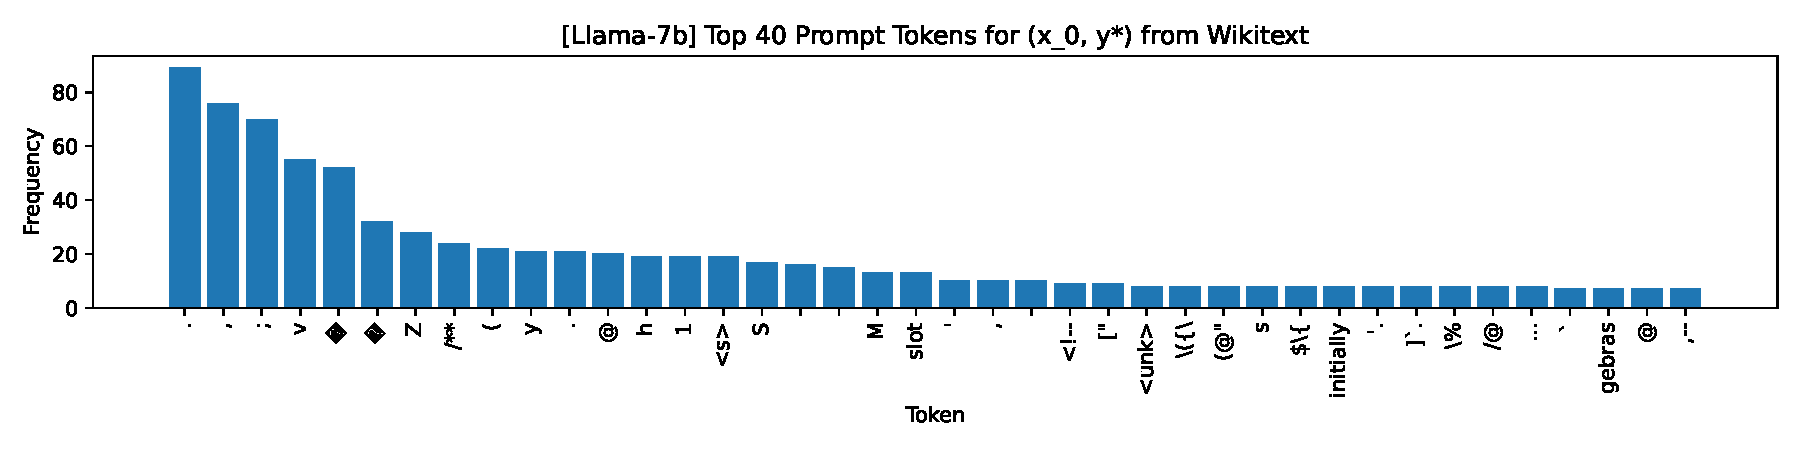
\includegraphics[width=0.9\textwidth]{figs/og_llama7b_prompt_token_freqs.pdf}
    }
    \subfigure[Falcon-40b]{
        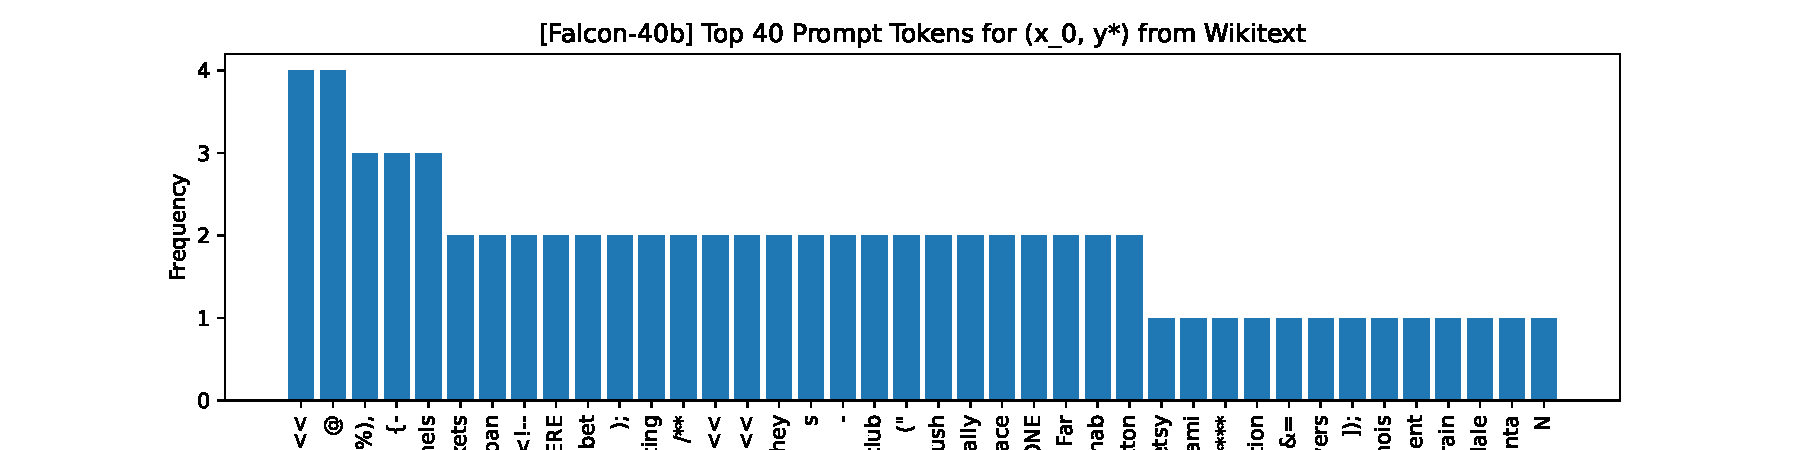
\includegraphics[width=0.9\textwidth]{figs/og_falcon40b_prompt_token_freqs.pdf}
    }
    \caption{Prompt token frequencies for Falcon-7b (top), Llama-7b (middle), and Falcon-40b (bottom) from Wikitext ground truth target token $k-\epsilon$ controllability experiments.}
    \label{fig:main_freqs}
\end{figure}



\subsection{Top-75 Wikitext Controllability Results} 
\label{sec:sup_75}
This subsection includes supplementary figures for the controllability of Llama-7b, Falcon-7b, and Falcon-40b on the Wikitext dataset where the target output token $y$ for a given initial state token sequence $\mathbf x_0$ is sampled uniformly from the top 75 highest-probability tokens as determined by the language model itself $P_{LM}(y | \mathbf x_0)$. 
Specifically, the dataset $\mathcal D$ consists of 25 unique initial state token sequences $\mathbf x_0$ sampled from Wikitext, each replicated 75 times for the top 75 most probable subsequent tokens $y \sim P(y | \mathbf x_0)$. 
This procedure yielded a dataset of 1875 initial state-target output pairs $(\mathbf x_0, y)$ for the 7 billion parameter models.
Due to the computational requirements for the 40 billion parameter model, the number of unique initial state token sequences was decreased to 10, resulting in a dataset of 750 initial state-target output pairs. 
The $k-\epsilon$ plots for each model are shown in Figure~\ref{fig:k_eps_75}. On average, across the 3 models, the top 75 outputs were reachable 86.865\% of the time with $k\leq 10$ prompt tokens. 
Similar log-linear trends were observed in the $k-\epsilon$ plot.
Figure~\ref{fig:base_loss_k_75} shows the relationship between base loss and required prompt length, revealing a more dramatic ``exclusion zone'' in the top left, similar to main ``ground truth'' results in Figure~\ref{fig:base_loss_k_main}.
Finally, Figure~\ref{fig:75_freqs} plots a histogram of the 40 most common tokens observed in the optimized control input prompts from the top-75 experiments. 


\begin{figure}[ht]
    \centering
    % First figure (on the left)
    \begin{minipage}[b]{0.48\textwidth}
        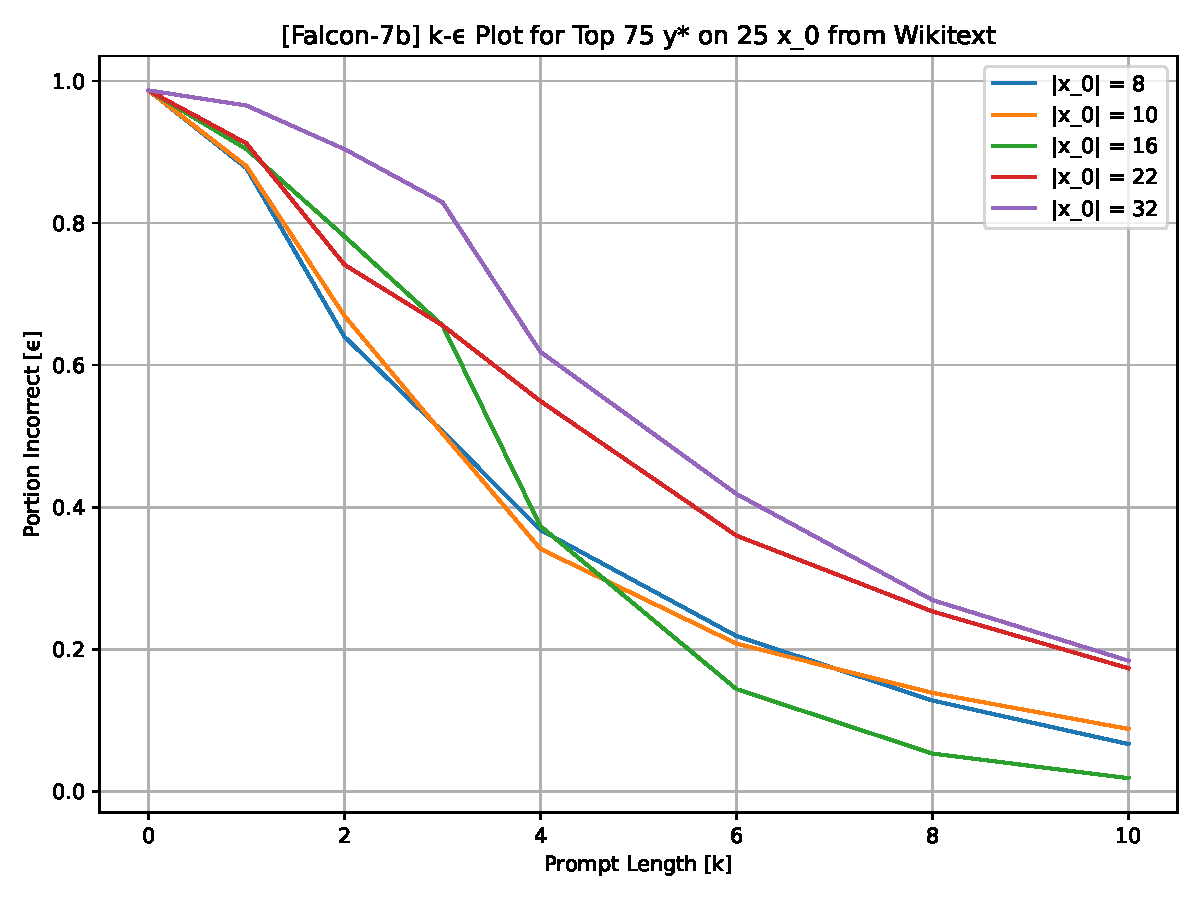
\includegraphics[width=\textwidth]{figs/shallow1_falcon7b_k_epsilon.pdf}
    \end{minipage}
    \hfill
    % Second figure (on the right)
    \begin{minipage}[b]{0.48\textwidth}
        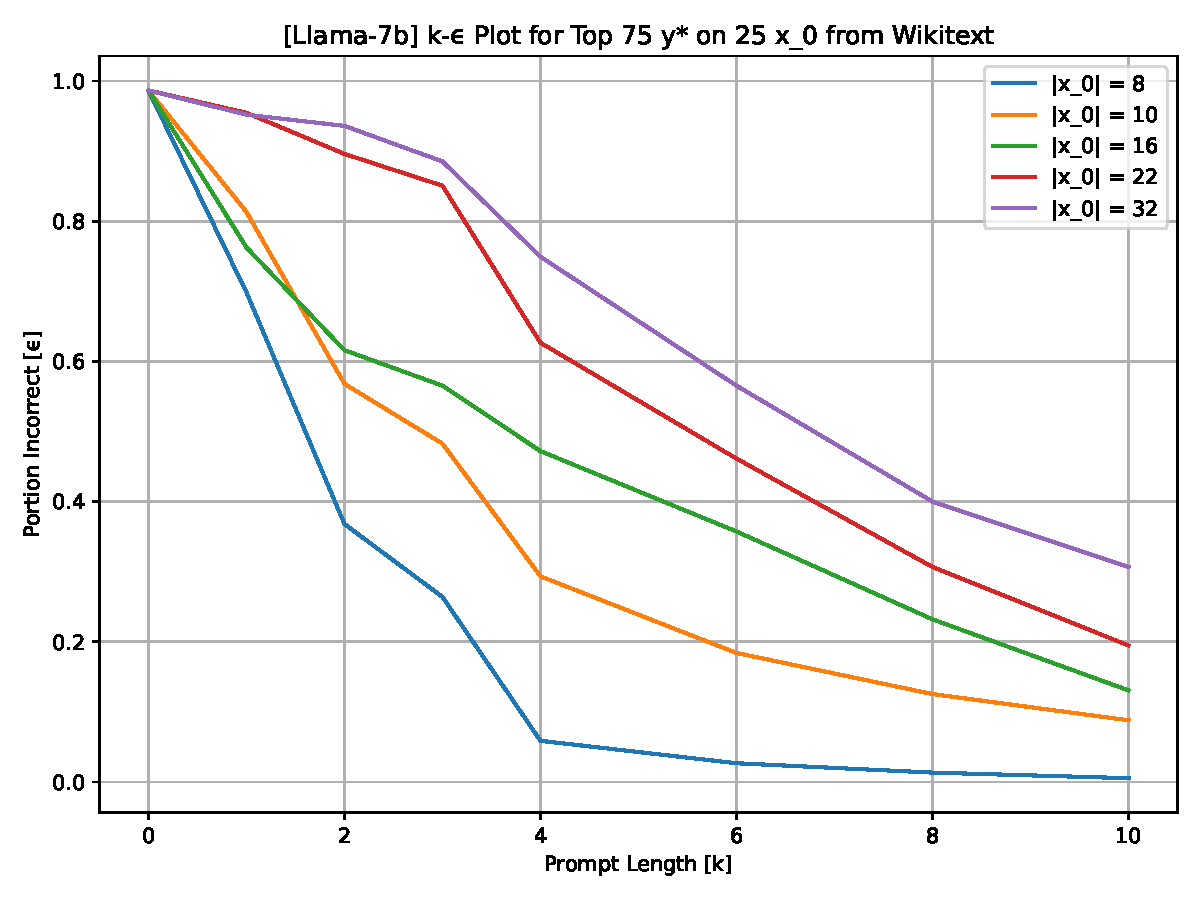
\includegraphics[width=\textwidth]{figs/shallow1_llama7b_k_epsilon.pdf}
    \end{minipage}
    \vspace{1em} % Optional: add a bit of vertical space between the rows
    % Collective caption in the fourth quadrant
    \begin{minipage}[b]{0.48\textwidth}
        \caption{
            $k-\epsilon$ controllability plots on the top 75 most likely output tokens.  \\
            \textbf{Top left}: $k-\epsilon$ values for Falcon-7b. With $k=10$ control tokens, 89.387\% of the top 75 output tokens were reachable. \\
            \textbf{Top right}: $k-\epsilon$ values for Llama-7b. With $k=10$ control tokens, 85.493\% of the top 75 output tokens were reachable. \\
            \textbf{Bottom right}: $k-\epsilon$ values for Falcon-40b. With $k=10$ control tokens, 85.714\% of the top 75 output tokens were reachable.
            \label{fig:k_eps_75}
        }
    \end{minipage}
    \hfill
    % Third figure (below the second)
    \begin{minipage}[b]{0.48\textwidth}
        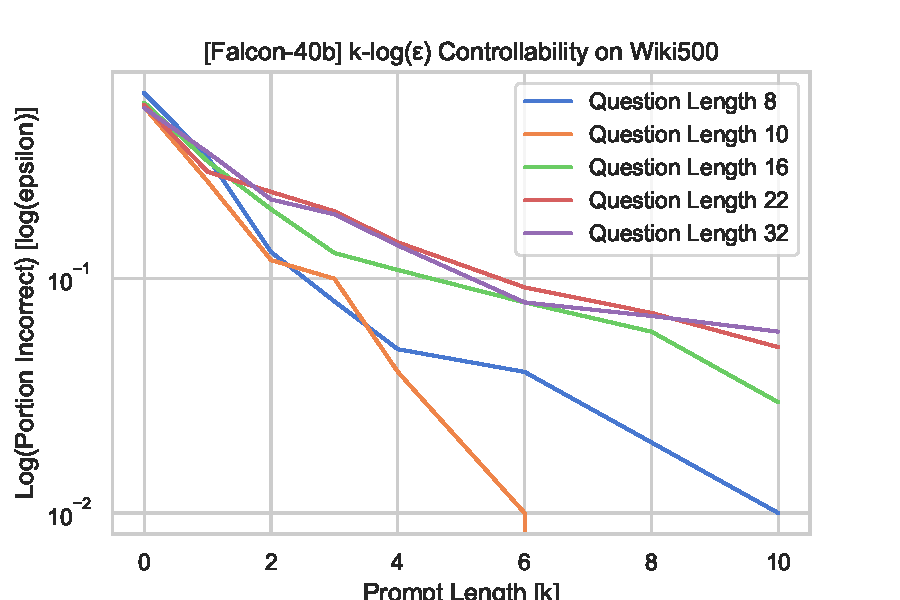
\includegraphics[width=\textwidth]{old_figs/falcon_40b/log_line_plot.pdf}
    \end{minipage}
\end{figure}


\begin{figure}[ht]
    \centering
    % First figure (on the left)
    \begin{minipage}[b]{0.48\textwidth}
        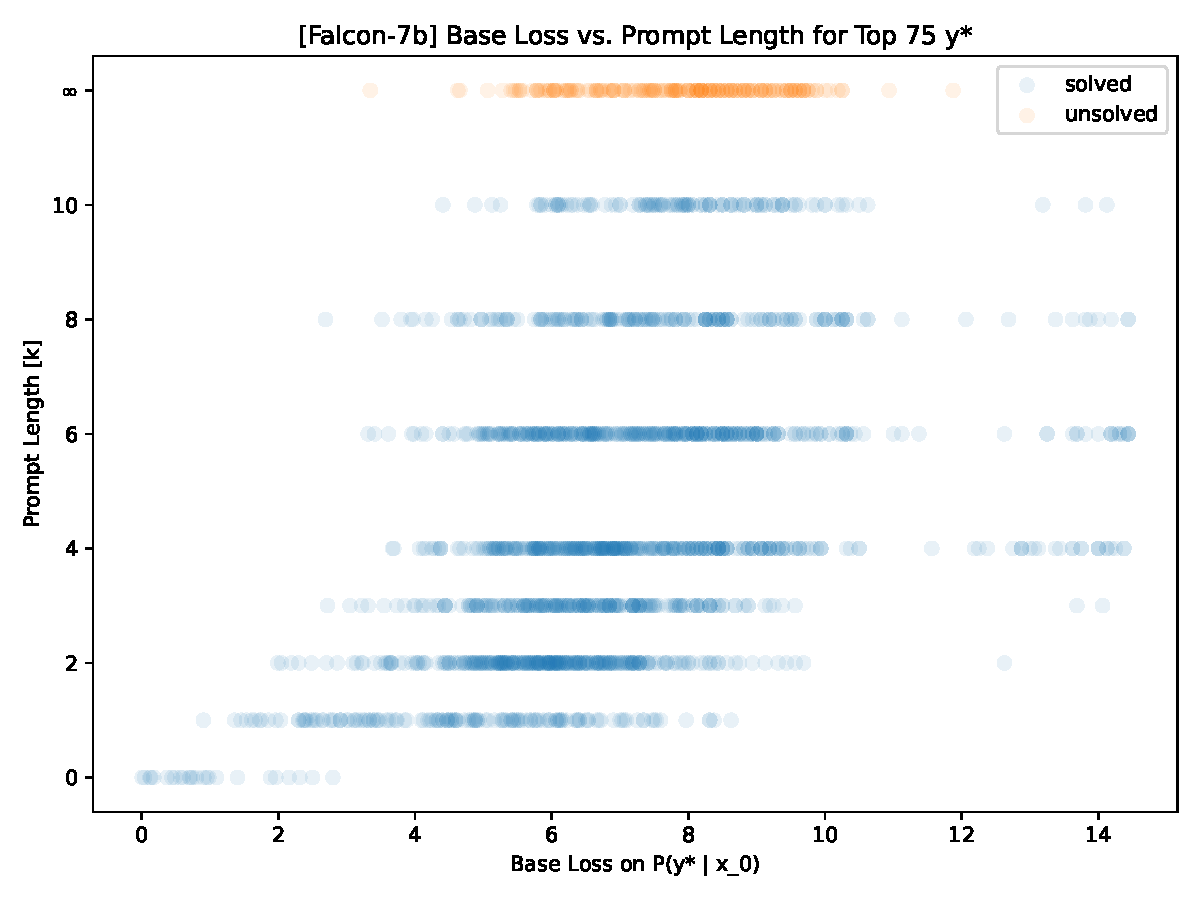
\includegraphics[width=\textwidth]{figs/shallow1_falcon7b_base_loss_vs_prompt_length.pdf}
    \end{minipage}
    \hfill
    % Second figure (on the right)
    \begin{minipage}[b]{0.48\textwidth}
        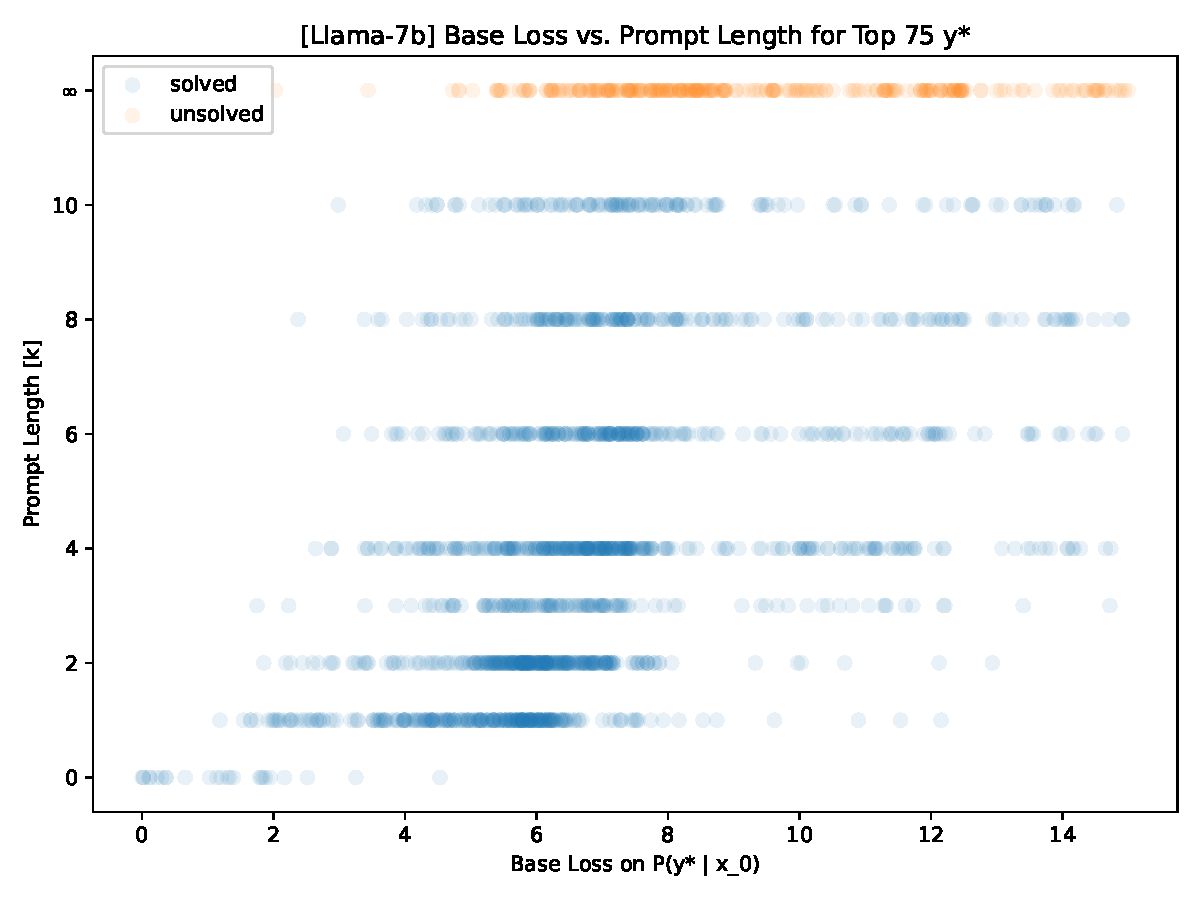
\includegraphics[width=\textwidth]{figs/shallow1_llama7b_base_loss_vs_prompt_length.pdf}
    \end{minipage}
    
    \vspace{1em} % Optional: add a bit of vertical space between the rows
    
    
    % Collective caption in the fourth quadrant
    \begin{minipage}[b]{0.48\textwidth}
        \caption{
            Required prompt length $k$ versus base loss on the target output $\mathcal L = -\log P_{LM}(y | \mathbf x_0)$ on synthetic top-75 dataset.
            While there does appear to be an ``exclusion zone'' in the top left-hand corner where a high prompt length is never associated with a base loss below a given threshold, base loss appears to be a poor predictor of required prompt length.
            \label{fig:base_loss_k_75}
        }
    \end{minipage}
    \hfill
    % Third figure (below the second)
    \begin{minipage}[b]{0.48\textwidth}
        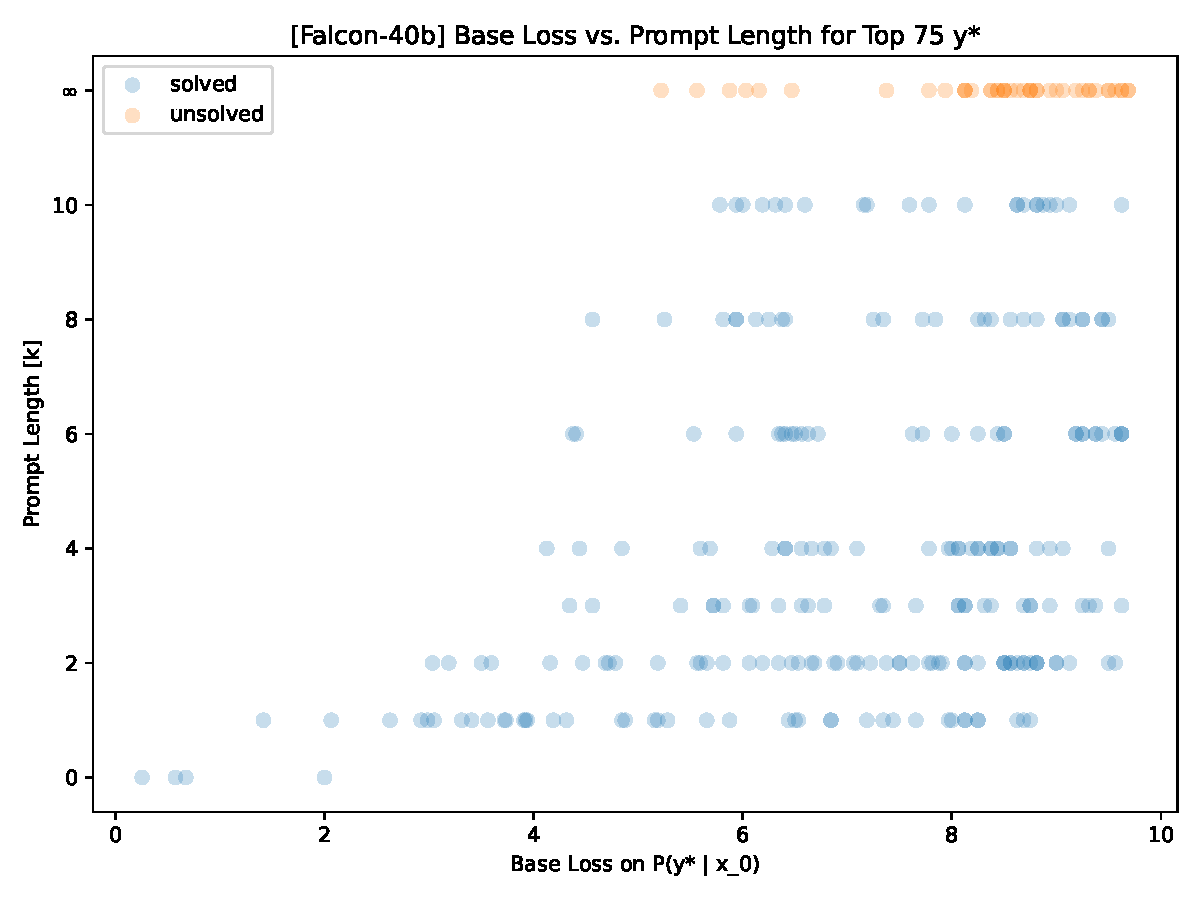
\includegraphics[width=\textwidth]{figs/shallow1_falcon40b_base_loss_vs_prompt_length.pdf}
    \end{minipage}
\end{figure}


\begin{figure}[htbp]
    \centering
    \subfigure[Falcon-7b]{
        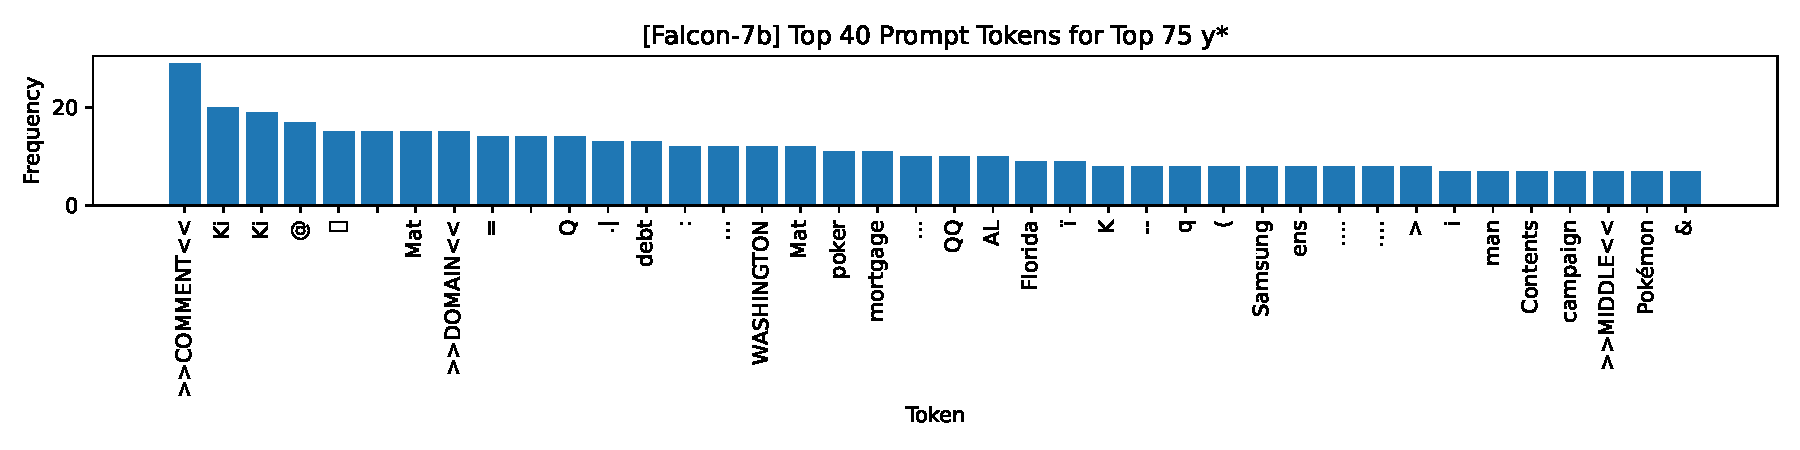
\includegraphics[width=0.9\textwidth]{figs/shallow1_falcon7b_prompt_token_freqs.pdf}
    }
    \subfigure[Llama-7b]{
        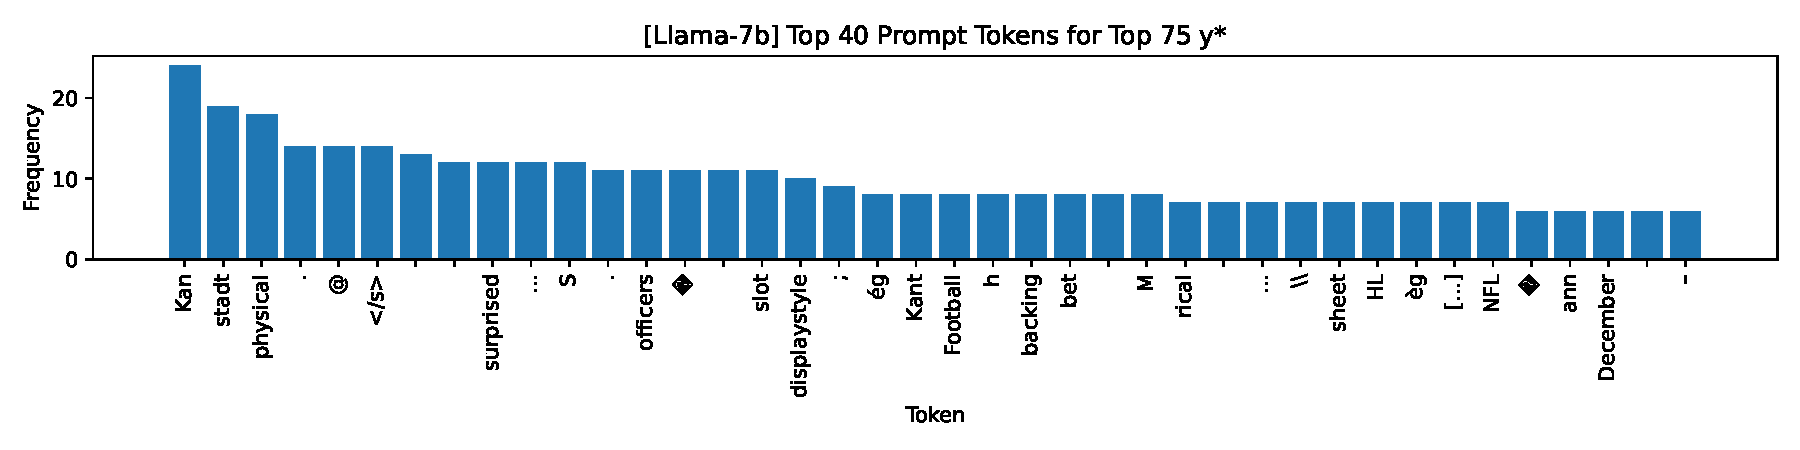
\includegraphics[width=0.9\textwidth]{figs/shallow1_llama7b_prompt_token_freqs.pdf}
    }
    \subfigure[Falcon-40b]{
        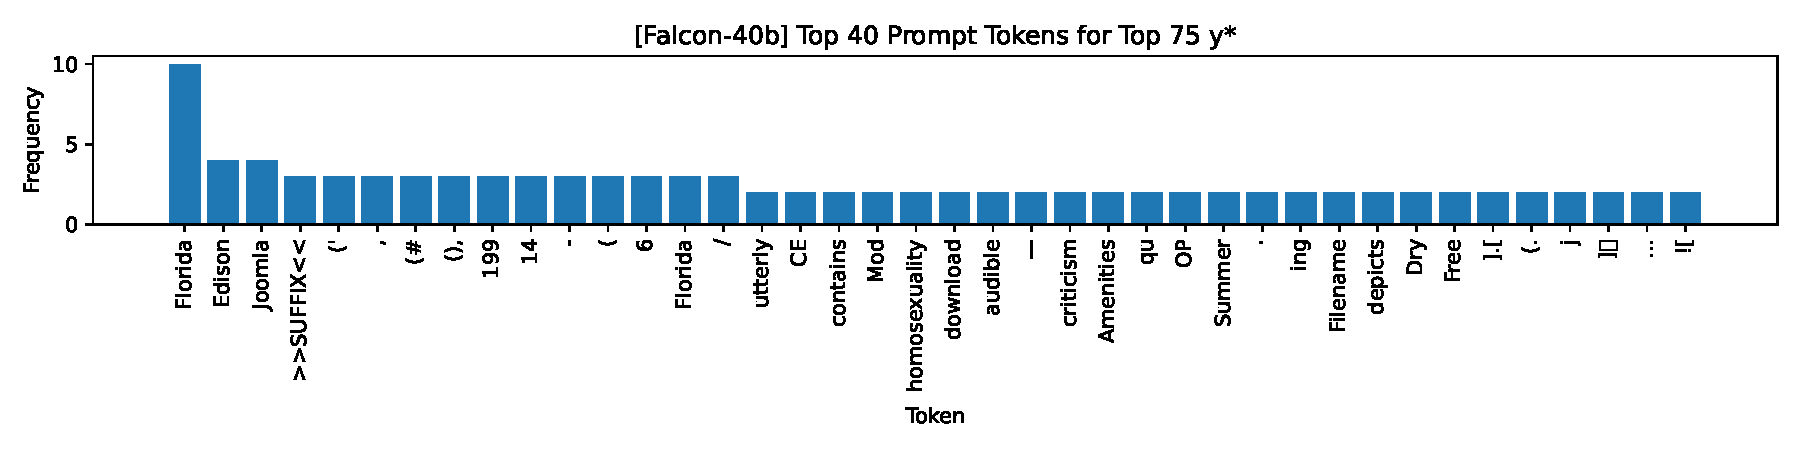
\includegraphics[width=0.9\textwidth]{figs/shallow1_falcon40b_prompt_token_freqs.pdf}
    }
    \caption{Prompt token frequencies for Falcon-7b (top), Llama-7b (middle), and Falcon-40b (bottom) from Wikitext top-75 synthetic dataset $k-\epsilon$ controllability experiments.}
    \label{fig:75_freqs}
\end{figure}












\subsection{Uniformly Sampled Output Token Results}
\label{sec:sup_deep}

This section contains supplementary figures for $k-\epsilon$ controllability experiments on a synthetic dataset $\mathcal D = \{(\mathbf x_0, y)\}$ where $\mathbf x_0$ are sampled from the Wikitext dataset and $y$ is sampled uniformly from the vocabulary. 
The uniform target output dataset $\mathcal D$ consists of 616 state-output pairs. 
Due to computational constraints, $k-\epsilon$ controllability was only measured for Falcon-7b. 
Overall, only 46.42\% of the target outputs were reachable with $k=10$ prompt tokens. 
Figure~\ref{fig:deep_main} visualizes the $k-\epsilon$ results, the relationship between base loss and prompt length, and the most frequently observed tokens in the optimized control prompts. 
While the ``exclusion zone'' behavior (cf Figures~\ref{fig:base_loss_k_75}, \ref{fig:base_loss_k_main}) is observed in the base loss vs. prompt length subplot, base loss remains a poor predictor of required prompt length. 
Moreover, Figure~\ref{fig:deep_falcon_rank_k} reveals an even more uniform relationship between the initial rank of the target output token and the required prompt length. 

% fig:deep_main
\begin{figure}[htbp]
    \centering
    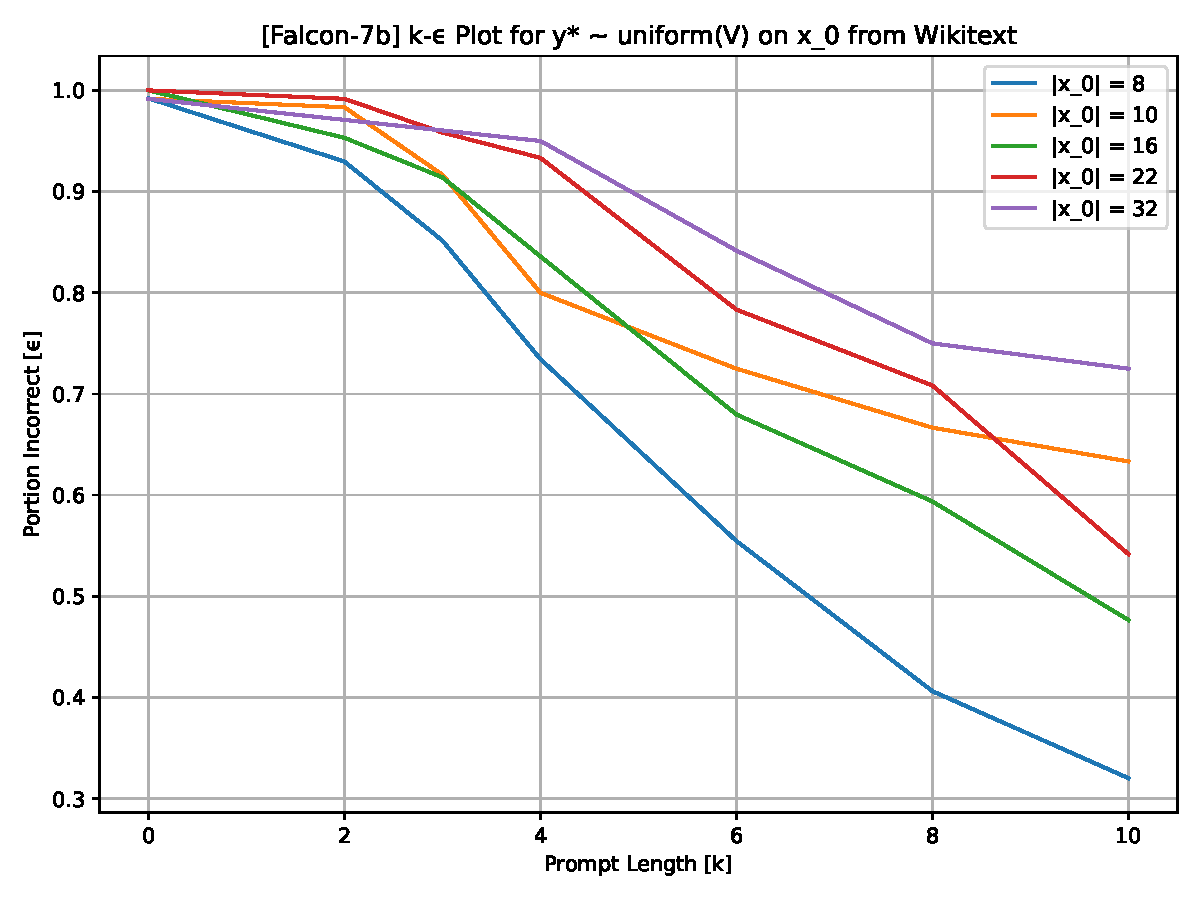
\includegraphics[width=0.48\linewidth]{figs/deep1_falcon7b_k_epsilon.pdf}
    \hfill
    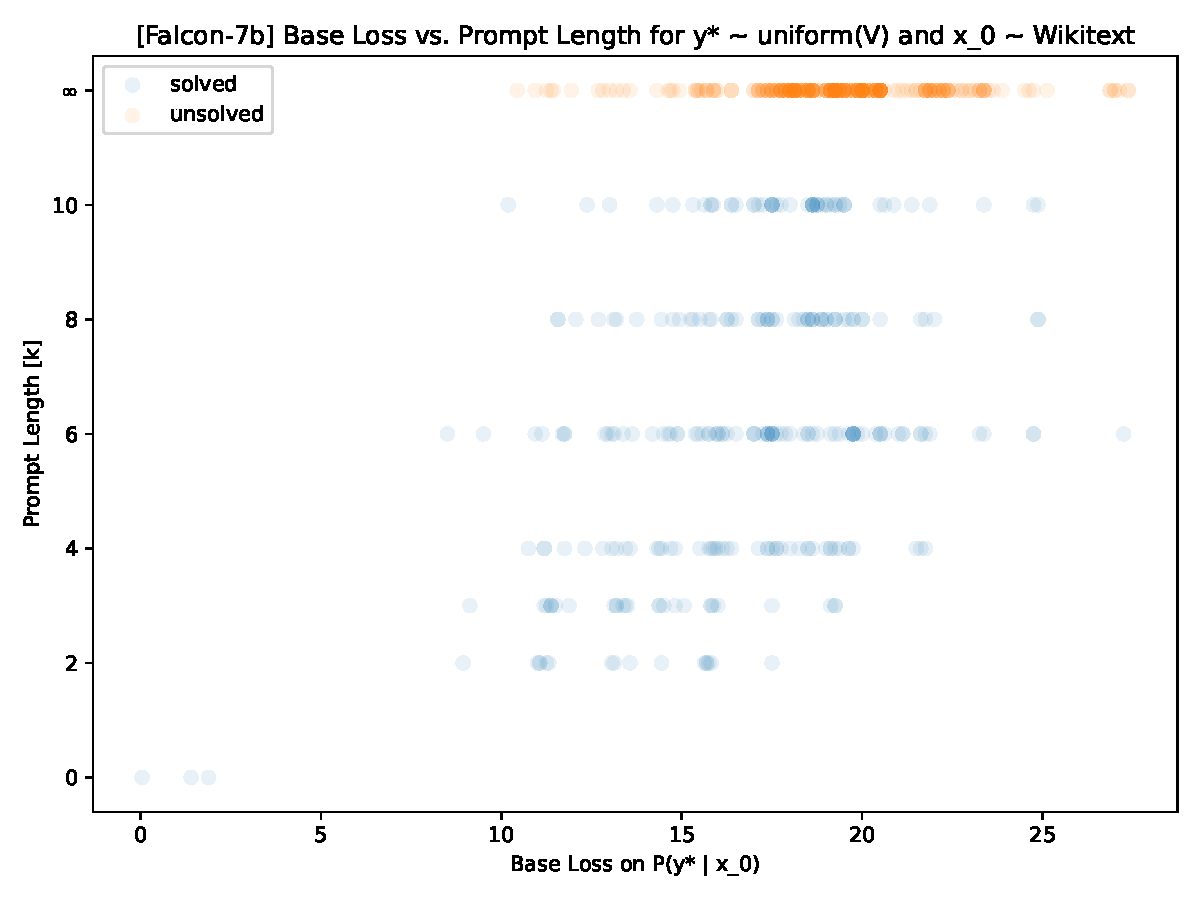
\includegraphics[width=0.48\linewidth]{figs/deep1_falcon7b_base_loss_vs_prompt_length.pdf}
    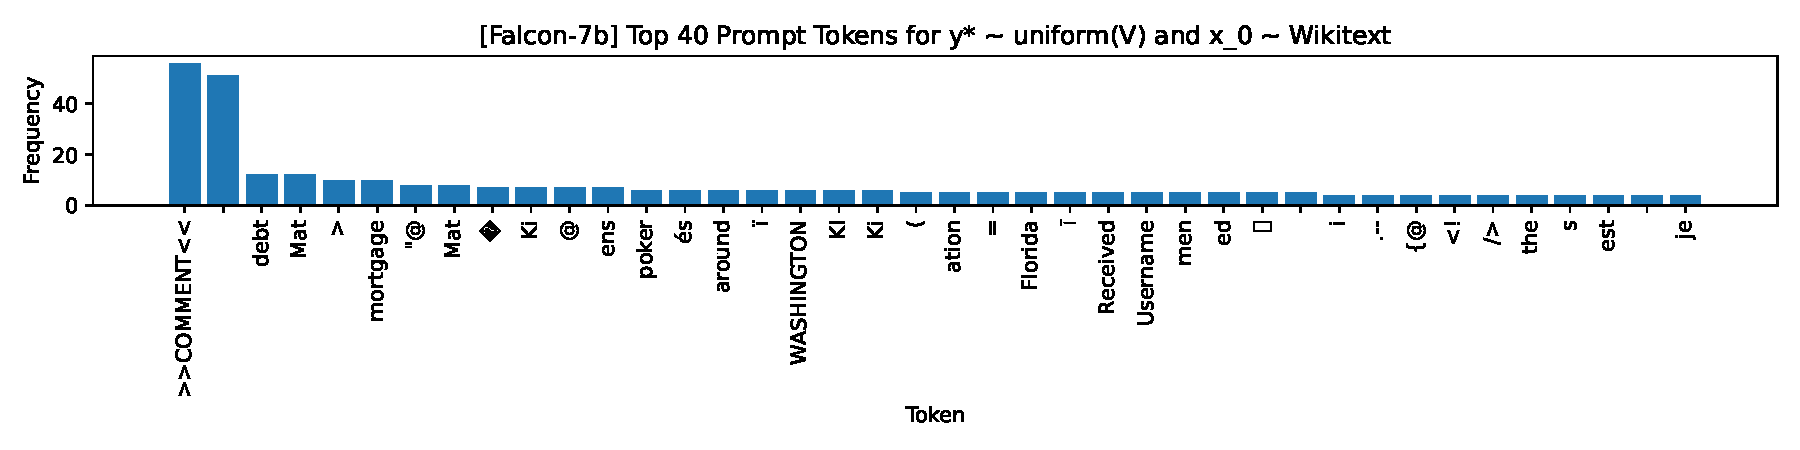
\includegraphics[width=\linewidth]{figs/deep1_falcon7b_prompt_token_freqs.pdf}
    \caption{Supplementary figures on uniformly sampled target output controllability tests on Falcon-7b. \textbf{Top Left:} $k-\epsilon$ plot (46.42\% controllable at $k=10$). \textbf{Top Right:} Base loss versus required prompt length. \textbf{Bottom:} Histogram of top 40 most frequent tokens in optimized control prompts.}
    \label{fig:deep_main}
\end{figure}






% \newpage
% \section{Control Definitions from Literature}
% \subsection{Kalman's definitions of Reachability and Controllability}
% \subsubsection{Kalman's Original Notation}

% % Reachability

% \textbf{Definition: Reachability} An event $(t, x)$ in a linear system $\Sigma$ is said to be reachable (from the zero state) iff there is some time $s \leq t$ and some input $\omega$ which carries $(s, 0)$ into $(t, x)$.


% % Controllability

% \textbf{Definition: Controllability } An event $(t, x)$ in a linear system $\Sigma$ is controllable (to the zero state) iff there is some time $t' \geq t$ and some input $\omega$ which carries $(t, x)$ into $(t', 0)$.

% \textbf{Definition: Complete Reachability and Controllability } We speak of complete reachability (or complete controllability) at time $\tau$ iff every event $(\tau, x)$, where $\tau$ is fixed and $x \in \mathcal{X}$, is reachable (or controllable). If the time $\tau$ is not mentioned, these properties must hold for all $\tau$.

% \cite{kalman1969topics}

% \subsubsection{Our notation based on abstract systems}
% % Reachability

% \textbf{Definition: Reachability } Given a system $\Sigma = (\mathcal{T, X, U}, \phi)$, a state $x \in \mathcal X$ at time $t \in \mathcal T$ is reachable from the zero state if there exists a time $s \in \mathcal T$ with $s \leq t$ and an input $u \in \mathcal U$ such that $\phi(0, u, s, t) = x$.

% \textbf{Definition: Complete Reachability } A system $\Sigma = (\mathcal{T, X, U}, \phi)$ exhibits complete reachability at time $\tau \in \mathcal{T}$ if for every $x \in \mathcal{X}$ there exists a time $s \in \mathcal{T}$ with $s \leq \tau$ and an input $u \in \mathcal{U}$ such that $\phi(0, u, s, \tau) = x$. If the time $\tau$ is not specified, then this condition must hold for all $\tau \in \mathcal{T}$.


% % Controllability

% \textbf{Definition: Controllability } Given a system $\Sigma = (\mathcal{T, X, U}, \phi)$, a state $x \in \mathcal X$ at time $t \in \mathcal T$ is controllable to the zero state if there exists a time $t' \in \mathcal T$ with $t' \geq t$ and an input $u \in \mathcal U$ such that $\phi(x, u, t, t') = 0$.

% \textbf{Definition: Complete Controllability } A system $\Sigma = (\mathcal{T, X, U}, \phi)$ exhibits complete controllability at time $\tau \in \mathcal{T}$ if for every $x \in \mathcal{X}$ there exists a time $t' \in \mathcal{T}$ with $t' \geq \tau$ and an input $u \in \mathcal{U}$ such that $\phi(x, u, \tau, t') = 0$. If the time $\tau$ is not specified, then this condition must hold for all $\tau \in \mathcal{T}$.

% \subsection{Ogata's definitions of State Controllability and Output Controllability}

% \subsubsection{Ogata's original notation}
% \textbf{Definition: State Controllability } Consider the continuous-time system described by the differential equation $\dot{x} = \mathbf{A}x + \mathbf{B}u$, where $x$ is the state vector, $u$ is the control signal, $\mathbf{A}$ is an \(n \times n\) matrix, and $\mathbf{B}$ is an \(n \times 1\) matrix. The system is said to be state controllable at \(t = t_0\) if it is possible to construct an unconstrained control signal that will transfer an initial state to any final state in a finite time interval \(t_0 \leq t \leq t_1\).

% \textbf{Definition: Complete State Controllability } The system described by the same equation is said to be completely state controllable if every state is controllable.

% \textbf{Definition: Output Controllability.} Consider the system described by
% \begin{align}
%     \dot{x} &= \mathbf{A}x + \mathbf{B}u \\
%     y &= \mathbf{C}x + \mathbf{D}u
% \end{align}
% where \( x \) is the state vector (\(n\)-vector), \( u \) is the control vector (\(r\)-vector), \( y \) is the output vector (\(m\)-vector), \( \mathbf{A} \) is an \( n \times n \) matrix, \( \mathbf{B} \) is an \( n \times r \) matrix, \( \mathbf{C} \) is an \( m \times n \) matrix, and \( \mathbf{D} \) is an \( m \times r \) matrix.

% The system is output controllable at time \( t_0 \) if for a given initial output \( y(t_0) \) and any desired final output \( y(t_1) \), there exists a control vector \( u(t) \) that will achieve \( y(t_1) \) from \( y(t_0) \) in a finite time interval \( t_0 \leq t \leq t_1 \).


% \textbf{Definition: Complete Output Controllability }The system is said to be completely output controllable if it is possible to construct an unconstrained control vector \( u(t) \) that will transfer any given initial output \( y(t_0) \) to any final output \( y(t_1) \) in a finite time interval \( t_0 \leq t \leq t_1 \).

% \cite{ogata2010modern}

% \subsubsection{Our notation}

% \textbf{Definition: State Controllability } Given a system $\Sigma = (\mathcal{T, X, U}, \phi)$ with $\mathcal{T} = \mathbb{R}^+$, $\mathcal{X} = \mathbb{R}^n$, and $\mathcal{U} = \mathbb{R}^r$, the system is state controllable at time $\tau \in \mathcal{T}$ if for any initial state $x_0 \in \mathcal{X}$ and any final state $x_f \in \mathcal{X}$, there exists a control function $u: \mathcal{T} \to \mathcal{U}$ such that $\phi(x_0, u, \tau, t) = x_f$ for some $t \geq \tau$.

% \textbf{Definition: Complete State Controllability } The system $\Sigma$ is completely state controllable if the state controllability condition holds for every $x_0, x_f \in \mathcal{X}$.

% \textbf{Definition: Output Controllability } Given a system $\Sigma = (\mathcal{T, X, U, Y}, \phi, h)$ with $\mathcal{T} = \mathbb{R}^+$, $\mathcal{X} = \mathbb{R}^n$, $\mathcal{U} = \mathbb{R}^r$, and $\mathcal{Y} = \mathbb{R}^m$, the system is output controllable for a given initial output $y_0 \in \mathcal{Y}$ at time $\tau_0 \in \mathcal{T}$ if for any desired final output $y_f \in \mathcal{Y}$, there exists a control function $u: \mathcal{T} \to \mathcal{U}$ and a corresponding time $\tau_1 \in \mathcal{T}$ with $\tau_1 \geq \tau_0$ such that $h(\phi(x_0, u, \tau_0, \tau_1), u(\tau_1), \tau_1) = y_f$.

% \textbf{Definition: Complete Output Controllability } The system $\Sigma$ is completely output controllable if the output controllability condition holds for every $y_0 \in \mathcal{Y}$ and for all $\tau_0 \in \mathcal{T}$.



\end{document}

